\definecolor{opt}{HTML}{51B824}
\definecolor{amm}{HTML}{CC0000}

\section{Cruscotto di valutazione della qualità}
\subsection{Qualità del processo di Fornitura}
\subsubsection{1M-PV - Planned Value e 2M-EV - Earned Value}
%--------- GRAFICO -----------%
\begin{figure*}[!h]
    \centering
    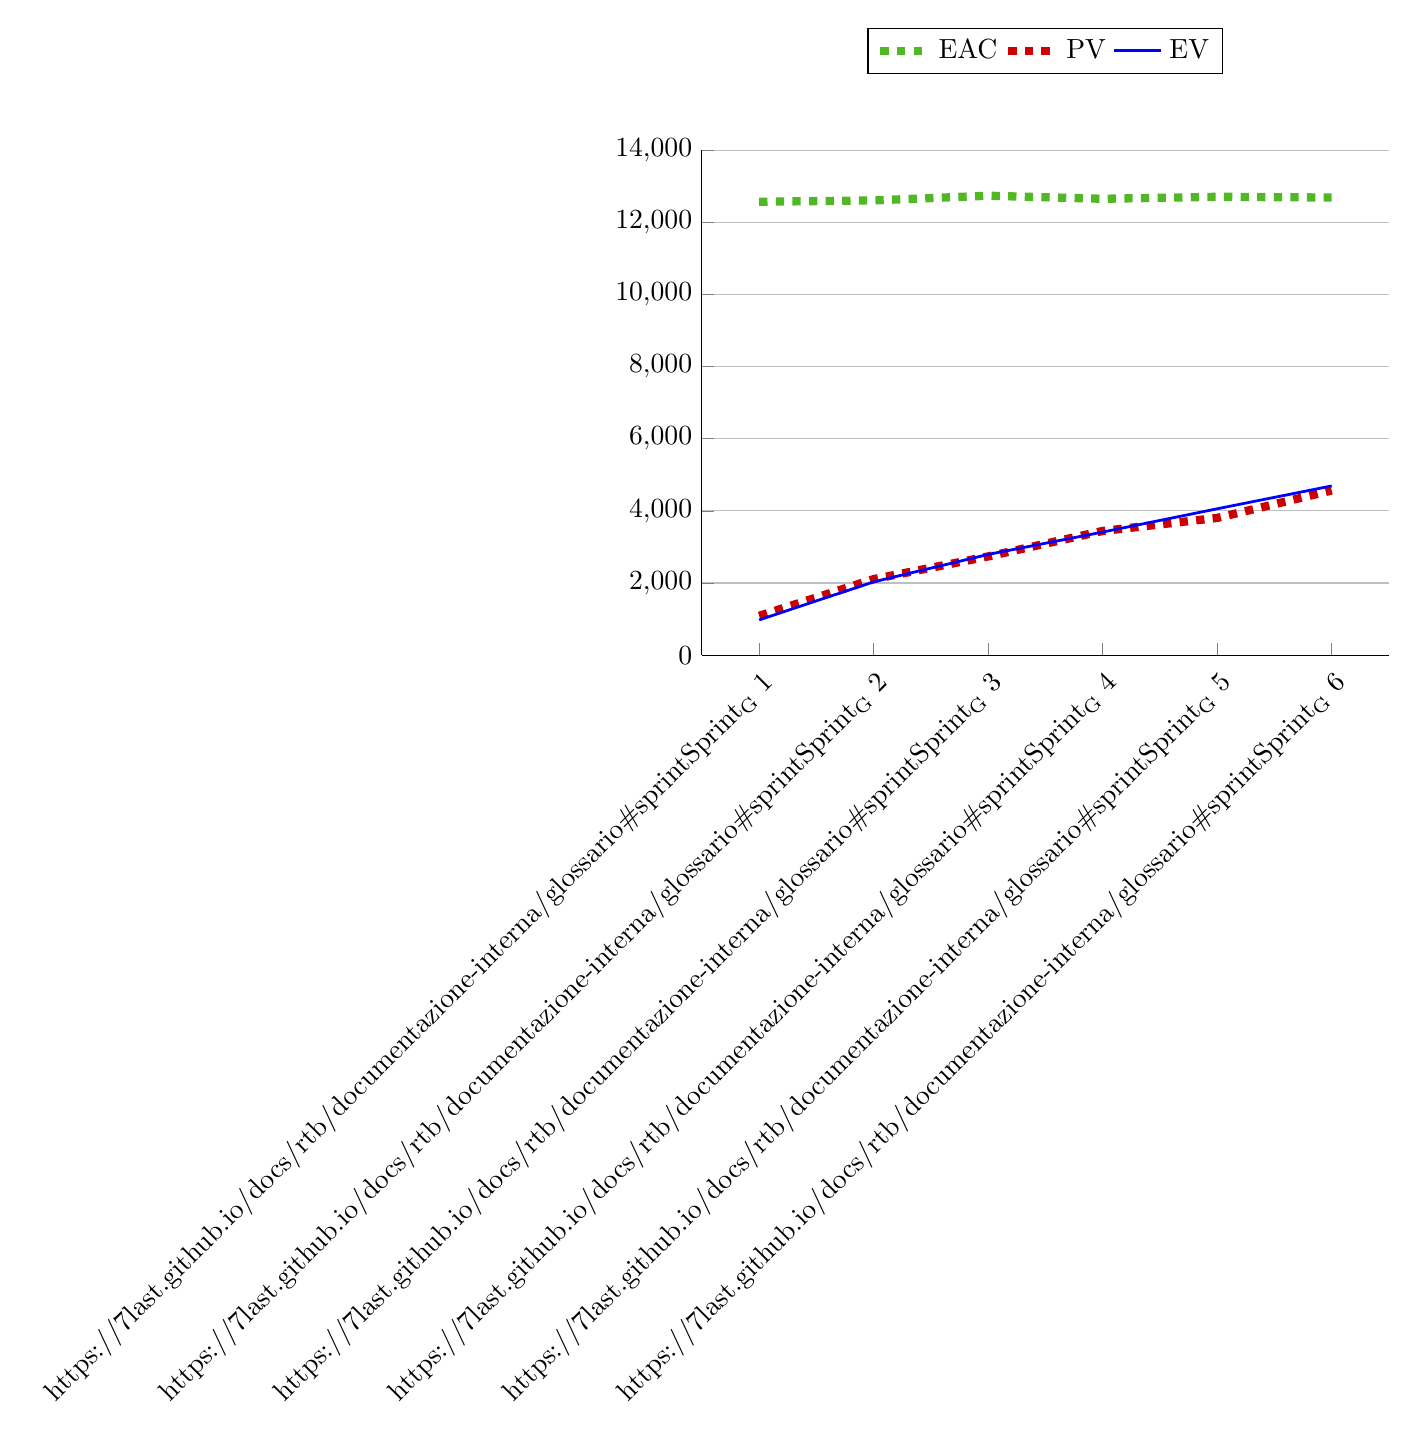
\begin{tikzpicture}
        \begin{axis}[
            width  = 0.85*\textwidth,
            height = 8cm,
            ymajorgrids = true,
            symbolic x coords={\href{https://7last.github.io/docs/rtb/documentazione-interna/glossario\#sprint}{Sprint\textsubscript{G}} 1, \href{https://7last.github.io/docs/rtb/documentazione-interna/glossario\#sprint}{Sprint\textsubscript{G}} 2, \href{https://7last.github.io/docs/rtb/documentazione-interna/glossario\#sprint}{Sprint\textsubscript{G}} 3, \href{https://7last.github.io/docs/rtb/documentazione-interna/glossario\#sprint}{Sprint\textsubscript{G}} 4, \href{https://7last.github.io/docs/rtb/documentazione-interna/glossario\#sprint}{Sprint\textsubscript{G}} 5, \href{https://7last.github.io/docs/rtb/documentazione-interna/glossario\#sprint}{Sprint\textsubscript{G}} 6},
            xtick = data,
            ymin=0,
            axis lines*=left,
            legend cell align=left,
            legend style={
                at={(0.5,1.15)},
                anchor=south,
                column sep=0.1ex,
                legend columns=3
            },
            xticklabel style={rotate=45, anchor=north east, yshift=0ex, xshift=0ex},
            scaled y ticks = false,
            yticklabel style={/pgf/number format/fixed}
        ]
            \addplot[color=opt, style={dashed, line width=3pt}, mark=none] coordinates {(\href{https://7last.github.io/docs/rtb/documentazione-interna/glossario\#sprint}{Sprint\textsubscript{G}} 1, 12567.5) (\href{https://7last.github.io/docs/rtb/documentazione-interna/glossario\#sprint}{Sprint\textsubscript{G}} 2, 12605) (\href{https://7last.github.io/docs/rtb/documentazione-interna/glossario\#sprint}{Sprint\textsubscript{G}} 3, 12735) (\href{https://7last.github.io/docs/rtb/documentazione-interna/glossario\#sprint}{Sprint\textsubscript{G}} 4, 12650) (\href{https://7last.github.io/docs/rtb/documentazione-interna/glossario\#sprint}{Sprint\textsubscript{G}} 5, 12705) (\href{https://7last.github.io/docs/rtb/documentazione-interna/glossario\#sprint}{Sprint\textsubscript{G}} 6, 12685)}; % EAC
            \addplot[color=amm, style={dashed, line width=3pt}, mark=none] coordinates {(\href{https://7last.github.io/docs/rtb/documentazione-interna/glossario\#sprint}{Sprint\textsubscript{G}} 1, 1090) (\href{https://7last.github.io/docs/rtb/documentazione-interna/glossario\#sprint}{Sprint\textsubscript{G}} 2, 2107.5) (\href{https://7last.github.io/docs/rtb/documentazione-interna/glossario\#sprint}{Sprint\textsubscript{G}} 3, 2737.5) (\href{https://7last.github.io/docs/rtb/documentazione-interna/glossario\#sprint}{Sprint\textsubscript{G}} 4, 3442.5) (\href{https://7last.github.io/docs/rtb/documentazione-interna/glossario\#sprint}{Sprint\textsubscript{G}} 5, 3804) (\href{https://7last.github.io/docs/rtb/documentazione-interna/glossario\#sprint}{Sprint\textsubscript{G}} 6, 4564.8)}; % PV
            \addplot[color=blue, style={line width=1pt}, mark=none] coordinates {(\href{https://7last.github.io/docs/rtb/documentazione-interna/glossario\#sprint}{Sprint\textsubscript{G}} 1, 977.5) (\href{https://7last.github.io/docs/rtb/documentazione-interna/glossario\#sprint}{Sprint\textsubscript{G}} 2, 2032.5) (\href{https://7last.github.io/docs/rtb/documentazione-interna/glossario\#sprint}{Sprint\textsubscript{G}} 3, 2792.5) (\href{https://7last.github.io/docs/rtb/documentazione-interna/glossario\#sprint}{Sprint\textsubscript{G}} 4, 3412.5) (\href{https://7last.github.io/docs/rtb/documentazione-interna/glossario\#sprint}{Sprint\textsubscript{G}} 5, 4057.6) (\href{https://7last.github.io/docs/rtb/documentazione-interna/glossario\#sprint}{Sprint\textsubscript{G}} 6, 4691.6)}; % EV
            \legend{EAC, PV, EV}
        \end{axis}
    \end{tikzpicture}
    \caption{Proiezione del PV e dell'EV}
\end{figure*}
%--------- FINE GRAFICO -----------%
\subsubsection*{\href{https://7last.github.io/docs/rtb/documentazione-interna/glossario\#requirements-and-technology-baseline}{RTB\textsubscript{G}}}
Visionando il grafico si può notare che i valori di EV e PV quasi si sovrappongono, questo indica la buona riuscita della pianificazione delle attività da parte del gruppo \textit{7Last}.
%TODO mettere considerazioni finali \href{https://7last.github.io/docs/rtb/documentazione-interna/glossario\#product-baseline}{PB\textsubscript{G}}

\newpage
\subsubsection{3M-AC - Actual Cost  e 9M-ETC - Estimate to Complete}
%--------- GRAFICO -----------%
\begin{figure*}[!h]
    \centering
    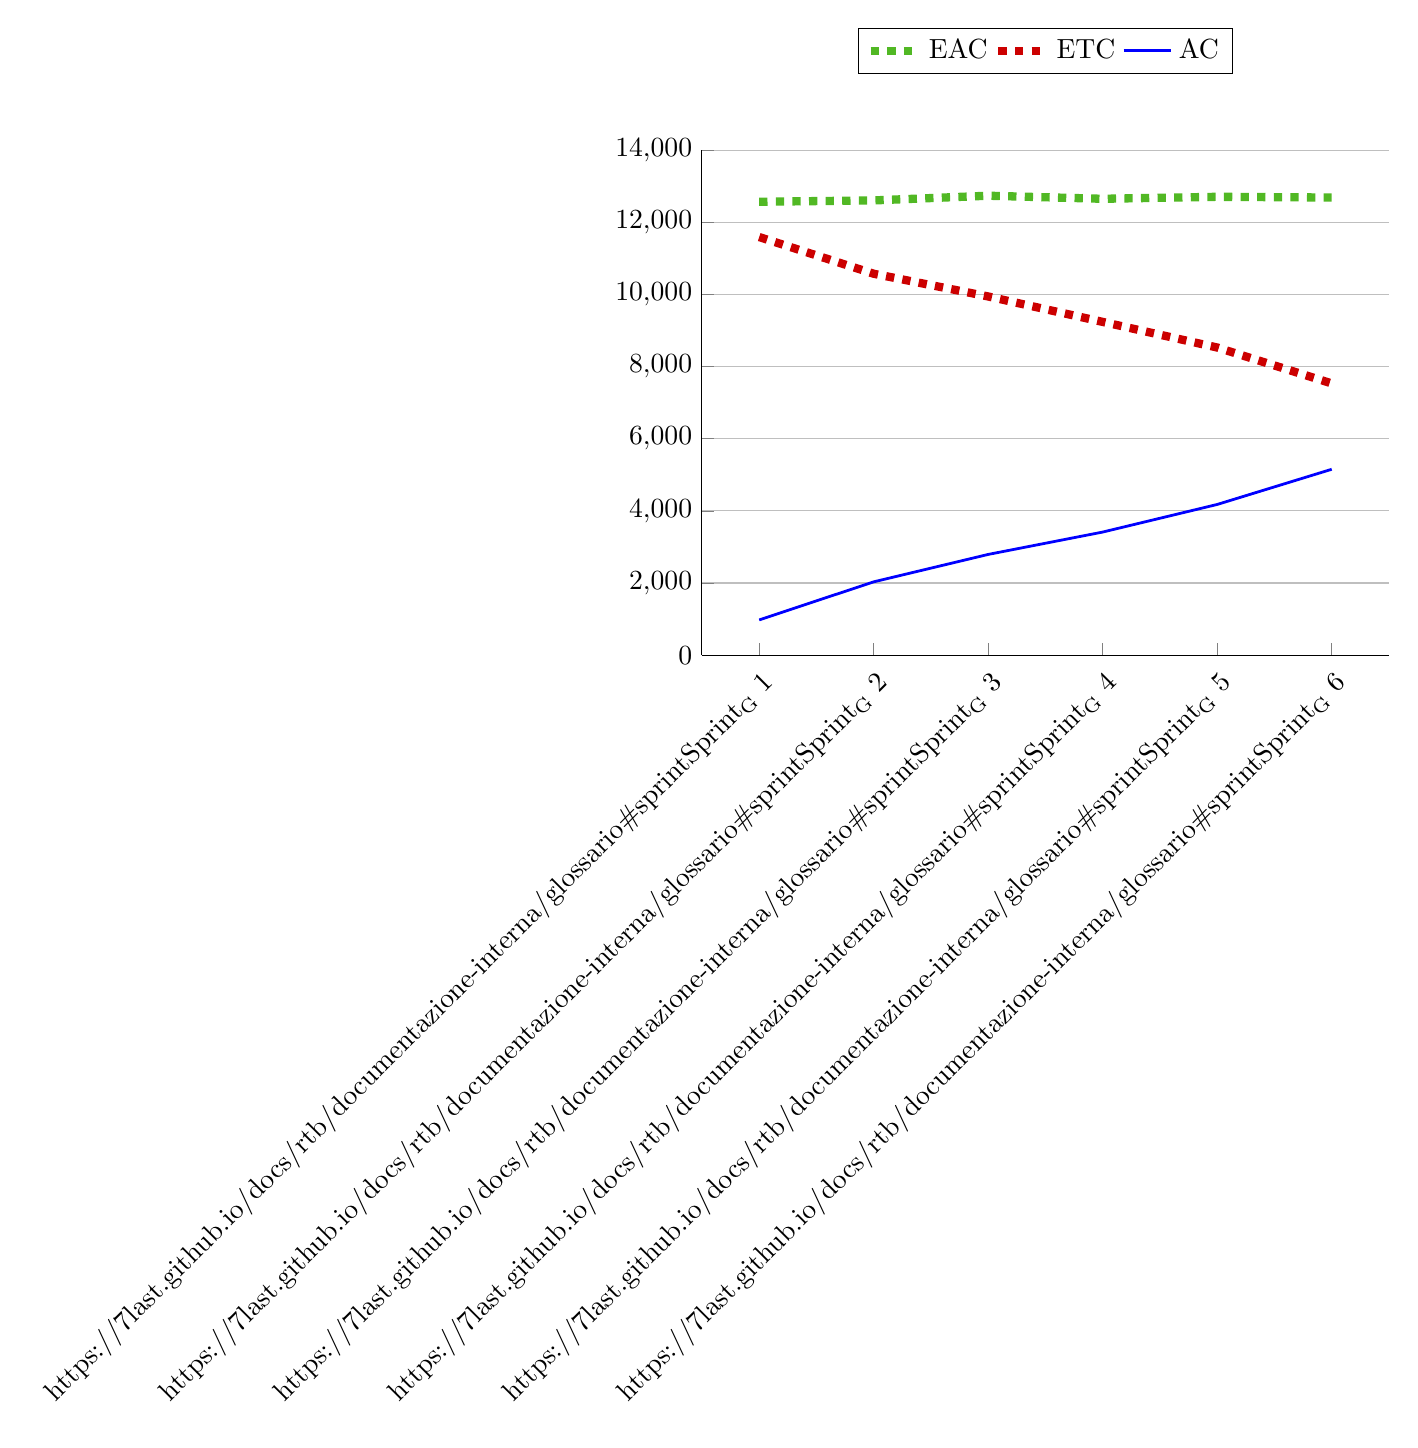
\begin{tikzpicture}
        \begin{axis}[
            width  = 0.85*\textwidth,
            height = 8cm,
            ymajorgrids = true,
            symbolic x coords={\href{https://7last.github.io/docs/rtb/documentazione-interna/glossario\#sprint}{Sprint\textsubscript{G}} 1, \href{https://7last.github.io/docs/rtb/documentazione-interna/glossario\#sprint}{Sprint\textsubscript{G}} 2, \href{https://7last.github.io/docs/rtb/documentazione-interna/glossario\#sprint}{Sprint\textsubscript{G}} 3, \href{https://7last.github.io/docs/rtb/documentazione-interna/glossario\#sprint}{Sprint\textsubscript{G}} 4, \href{https://7last.github.io/docs/rtb/documentazione-interna/glossario\#sprint}{Sprint\textsubscript{G}} 5, \href{https://7last.github.io/docs/rtb/documentazione-interna/glossario\#sprint}{Sprint\textsubscript{G}} 6},
            xtick = data,
            ymin=0,
            axis lines*=left,
            legend cell align=left,
            legend style={
                at={(0.5,1.15)},
                anchor=south,
                column sep=0.1ex,
                legend columns=3
            },
            xticklabel style={rotate=45, anchor=north east, yshift=0ex, xshift=0ex},
            scaled y ticks = false,
            yticklabel style={/pgf/number format/fixed}
        ]
            \addplot[color=opt, style={dashed, line width=3pt}, mark=none] coordinates {(\href{https://7last.github.io/docs/rtb/documentazione-interna/glossario\#sprint}{Sprint\textsubscript{G}} 1, 12567.5) (\href{https://7last.github.io/docs/rtb/documentazione-interna/glossario\#sprint}{Sprint\textsubscript{G}} 2, 12605) (\href{https://7last.github.io/docs/rtb/documentazione-interna/glossario\#sprint}{Sprint\textsubscript{G}} 3, 12735) (\href{https://7last.github.io/docs/rtb/documentazione-interna/glossario\#sprint}{Sprint\textsubscript{G}} 4, 12650) (\href{https://7last.github.io/docs/rtb/documentazione-interna/glossario\#sprint}{Sprint\textsubscript{G}} 5, 12705) (\href{https://7last.github.io/docs/rtb/documentazione-interna/glossario\#sprint}{Sprint\textsubscript{G}} 6, 12685)}; % EAC
            \addplot[color=amm, style={dashed, line width=3pt}, mark=none] coordinates {(\href{https://7last.github.io/docs/rtb/documentazione-interna/glossario\#sprint}{Sprint\textsubscript{G}} 1, 11590) (\href{https://7last.github.io/docs/rtb/documentazione-interna/glossario\#sprint}{Sprint\textsubscript{G}} 2, 10572.5) (\href{https://7last.github.io/docs/rtb/documentazione-interna/glossario\#sprint}{Sprint\textsubscript{G}} 3, 9942.5) (\href{https://7last.github.io/docs/rtb/documentazione-interna/glossario\#sprint}{Sprint\textsubscript{G}} 4, 9237.5) (\href{https://7last.github.io/docs/rtb/documentazione-interna/glossario\#sprint}{Sprint\textsubscript{G}} 5, 8527.5) (\href{https://7last.github.io/docs/rtb/documentazione-interna/glossario\#sprint}{Sprint\textsubscript{G}} 6, 7532.5)}; % ETC
            \addplot[color=blue, style={line width=1pt}, mark=none] coordinates {(\href{https://7last.github.io/docs/rtb/documentazione-interna/glossario\#sprint}{Sprint\textsubscript{G}} 1, 977.5) (\href{https://7last.github.io/docs/rtb/documentazione-interna/glossario\#sprint}{Sprint\textsubscript{G}} 2, 2032.5) (\href{https://7last.github.io/docs/rtb/documentazione-interna/glossario\#sprint}{Sprint\textsubscript{G}} 3, 2792.5) (\href{https://7last.github.io/docs/rtb/documentazione-interna/glossario\#sprint}{Sprint\textsubscript{G}} 4, 3412.5) (\href{https://7last.github.io/docs/rtb/documentazione-interna/glossario\#sprint}{Sprint\textsubscript{G}} 5, 4177.5) (\href{https://7last.github.io/docs/rtb/documentazione-interna/glossario\#sprint}{Sprint\textsubscript{G}} 6, 5152.5)}; % AC
            \legend{EAC, ETC, AC}
        \end{axis}
    \end{tikzpicture}
    \caption{Proiezione dell'AC e dell'ETC}
\end{figure*}
%--------- FINE GRAFICO -----------%
\subsubsection*{\href{https://7last.github.io/docs/rtb/documentazione-interna/glossario\#requirements-and-technology-baseline}{RTB\textsubscript{G}}}
Il grafico evidenzia chiaramente un aumento progressivo dei costi (AC). Parallelamente, si osserva una diminuzione della stima dei costi a finire (ETC), che sta calando in modo proporzionale all'incremento dei costi.

%TODO mettere considerazioni finali \href{https://7last.github.io/docs/rtb/documentazione-interna/glossario\#product-baseline}{PB\textsubscript{G}}
\newpage
\subsubsection{4M-SV - Schedule Variance e 5M-CV - Cost Variance}
%--------- GRAFICO -----------%
\begin{figure*}[!h]
    \centering
    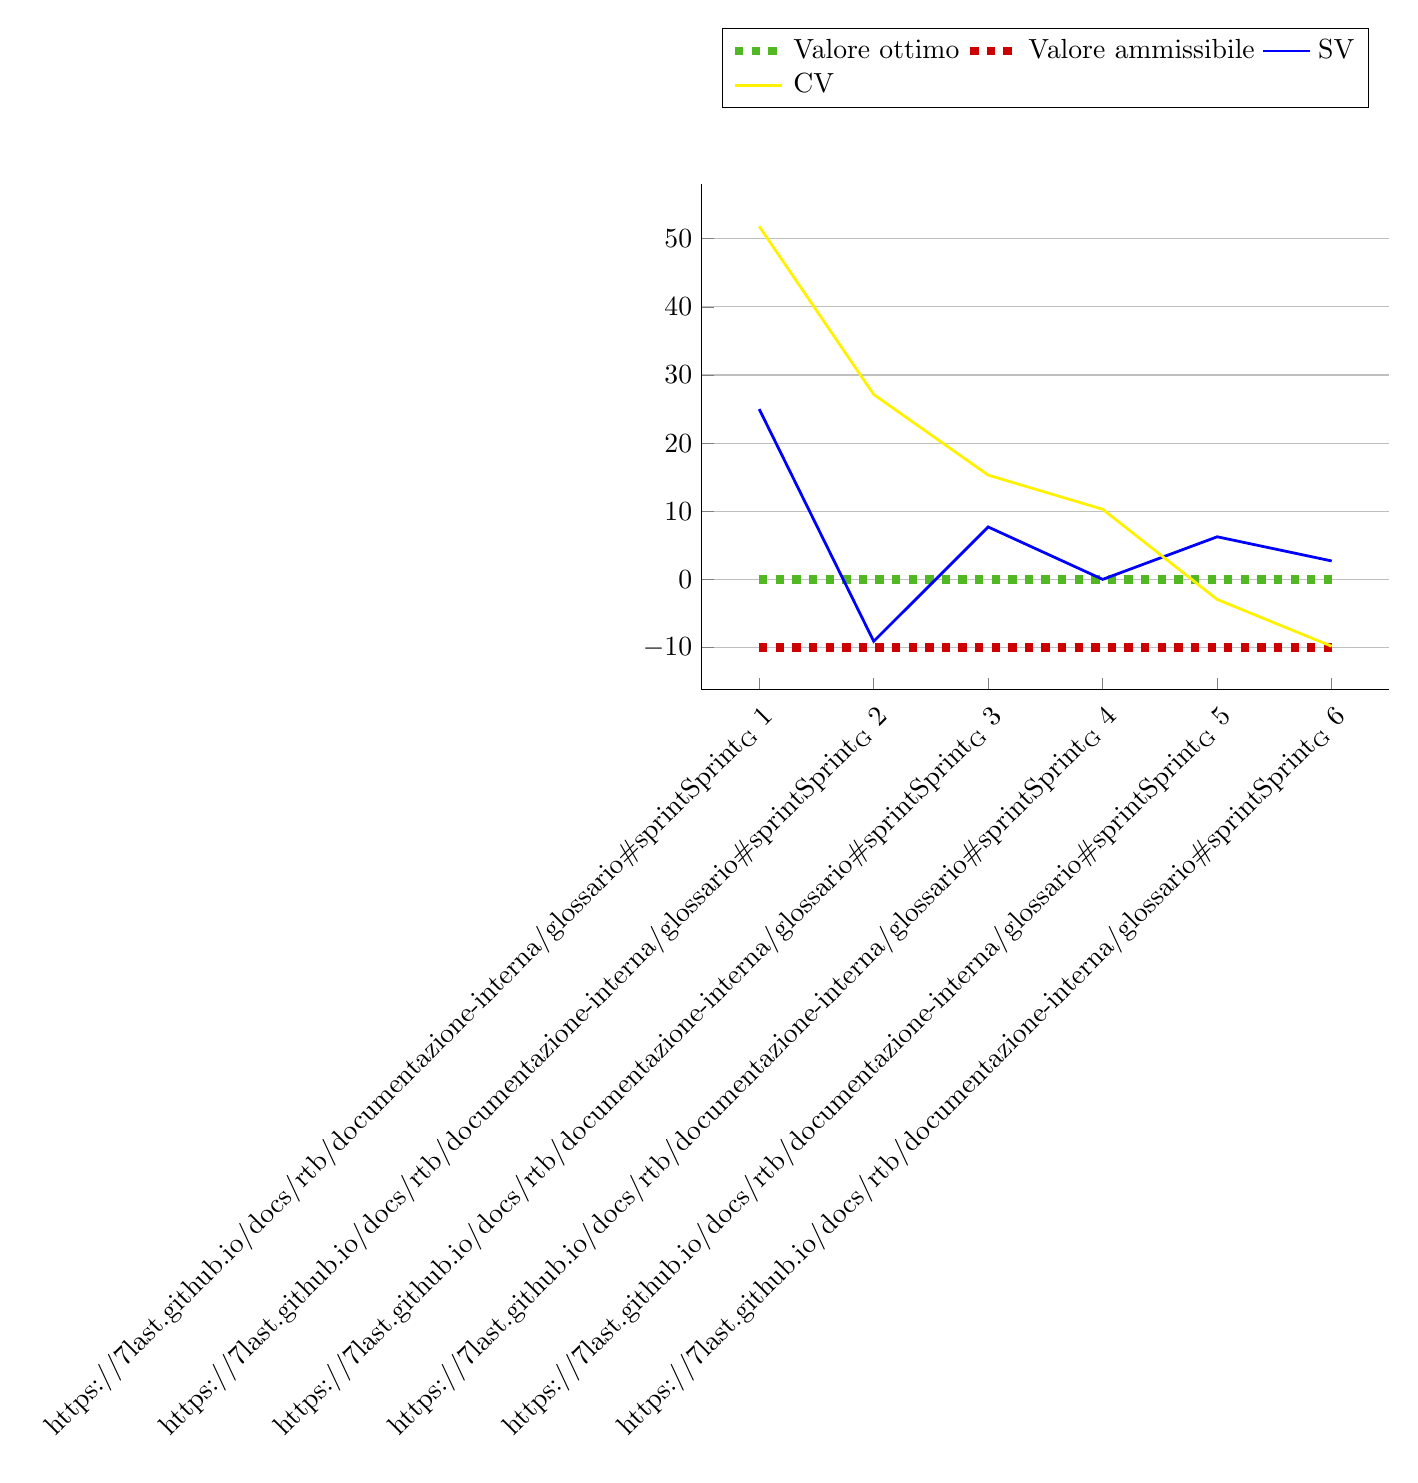
\begin{tikzpicture}
        \begin{axis}[
            width  = 0.85*\textwidth,
            height = 8cm,
            ymajorgrids = true,
            symbolic x coords={\href{https://7last.github.io/docs/rtb/documentazione-interna/glossario\#sprint}{Sprint\textsubscript{G}} 1, \href{https://7last.github.io/docs/rtb/documentazione-interna/glossario\#sprint}{Sprint\textsubscript{G}} 2, \href{https://7last.github.io/docs/rtb/documentazione-interna/glossario\#sprint}{Sprint\textsubscript{G}} 3, \href{https://7last.github.io/docs/rtb/documentazione-interna/glossario\#sprint}{Sprint\textsubscript{G}} 4, \href{https://7last.github.io/docs/rtb/documentazione-interna/glossario\#sprint}{Sprint\textsubscript{G}} 5, \href{https://7last.github.io/docs/rtb/documentazione-interna/glossario\#sprint}{Sprint\textsubscript{G}} 6},
            xtick = data,
            axis lines*=left,
            legend cell align=left,
            legend style={
                at={(0.5,1.15)},
                anchor=south,
                column sep=0.1ex,
                legend columns=3
            },
            xticklabel style={rotate=45, anchor=north east, yshift=0ex, xshift=0ex}
        ]
            \addplot[color=opt, style={dashed, line width=3pt}, mark=none] coordinates {(\href{https://7last.github.io/docs/rtb/documentazione-interna/glossario\#sprint}{Sprint\textsubscript{G}} 1, 0) (\href{https://7last.github.io/docs/rtb/documentazione-interna/glossario\#sprint}{Sprint\textsubscript{G}} 2, 0) (\href{https://7last.github.io/docs/rtb/documentazione-interna/glossario\#sprint}{Sprint\textsubscript{G}} 3, 0) (\href{https://7last.github.io/docs/rtb/documentazione-interna/glossario\#sprint}{Sprint\textsubscript{G}} 4, 0) (\href{https://7last.github.io/docs/rtb/documentazione-interna/glossario\#sprint}{Sprint\textsubscript{G}} 5, 0) (\href{https://7last.github.io/docs/rtb/documentazione-interna/glossario\#sprint}{Sprint\textsubscript{G}} 6, 0)}; % ottimo = 0
            \addplot[color=amm, style={dashed, line width=3pt}, mark=none] coordinates {(\href{https://7last.github.io/docs/rtb/documentazione-interna/glossario\#sprint}{Sprint\textsubscript{G}} 1, -10) (\href{https://7last.github.io/docs/rtb/documentazione-interna/glossario\#sprint}{Sprint\textsubscript{G}} 2, -10) (\href{https://7last.github.io/docs/rtb/documentazione-interna/glossario\#sprint}{Sprint\textsubscript{G}} 3, -10) (\href{https://7last.github.io/docs/rtb/documentazione-interna/glossario\#sprint}{Sprint\textsubscript{G}} 4, -10) (\href{https://7last.github.io/docs/rtb/documentazione-interna/glossario\#sprint}{Sprint\textsubscript{G}} 5, -10) (\href{https://7last.github.io/docs/rtb/documentazione-interna/glossario\#sprint}{Sprint\textsubscript{G}} 6, -10)}; % ammissibile = -10
            \addplot[color=blue, style={line width=1pt}, mark=none] coordinates {(\href{https://7last.github.io/docs/rtb/documentazione-interna/glossario\#sprint}{Sprint\textsubscript{G}} 1, 25) (\href{https://7last.github.io/docs/rtb/documentazione-interna/glossario\#sprint}{Sprint\textsubscript{G}} 2, -9.09) (\href{https://7last.github.io/docs/rtb/documentazione-interna/glossario\#sprint}{Sprint\textsubscript{G}} 3, 7.69) (\href{https://7last.github.io/docs/rtb/documentazione-interna/glossario\#sprint}{Sprint\textsubscript{G}} 4, 0) (\href{https://7last.github.io/docs/rtb/documentazione-interna/glossario\#sprint}{Sprint\textsubscript{G}} 5, 6.25) (\href{https://7last.github.io/docs/rtb/documentazione-interna/glossario\#sprint}{Sprint\textsubscript{G}} 6, 2.7)}; % SV
            \addplot[color=yellow, style={line width=1pt}, mark=none] coordinates {(\href{https://7last.github.io/docs/rtb/documentazione-interna/glossario\#sprint}{Sprint\textsubscript{G}} 1, 51.82) (\href{https://7last.github.io/docs/rtb/documentazione-interna/glossario\#sprint}{Sprint\textsubscript{G}} 2, 27.14) (\href{https://7last.github.io/docs/rtb/documentazione-interna/glossario\#sprint}{Sprint\textsubscript{G}} 3, 15.30) (\href{https://7last.github.io/docs/rtb/documentazione-interna/glossario\#sprint}{Sprint\textsubscript{G}} 4, 10.29) (\href{https://7last.github.io/docs/rtb/documentazione-interna/glossario\#sprint}{Sprint\textsubscript{G}} 5, -2.95) (\href{https://7last.github.io/docs/rtb/documentazione-interna/glossario\#sprint}{Sprint\textsubscript{G}} 6, -9.82)}; % CV
            \legend{Valore ottimo, Valore ammissibile, SV, CV}
        \end{axis}
    \end{tikzpicture}
    \caption{Andamento percentuale di SV e CV}
\end{figure*}
%--------- FINE GRAFICO -----------%
\subsubsection*{\href{https://7last.github.io/docs/rtb/documentazione-interna/glossario\#requirements-and-technology-baseline}{RTB\textsubscript{G}}}
Dal grafico si nota come sia SV che CV siano inizialmente elevati, per poi decrescere durante la prosecuzione del progetto, in particolare si nota un andamento altalenante del SV. \\
L'andamento inizialmente alto del Schedule Variance (SV) e del Cost Variance (CV) indica una possibile sovrastima iniziale dei tempi e dei costi, dovuta all'inesperienza del team. La variabilità del SV suggerisce che le stime di tempistiche iniziali erano eccessivamente conservative, con aggiustamenti successivi man mano che il team acquisiva esperienza. La decrescita nel tempo di entrambe le metriche mostra che il gruppo sta diventando più preciso nelle sue previsioni, con un allineamento progressivo dei costi e delle tempistiche reali rispetto a quelle pianificate.

%TODO mettere considerazioni finali \href{https://7last.github.io/docs/rtb/documentazione-interna/glossario\#product-baseline}{PB\textsubscript{G}}

\newpage
\subsubsection{8M-EAC - Estimated at Completion}
%--------- GRAFICO -----------%
\begin{figure*}[!h]
    \centering
    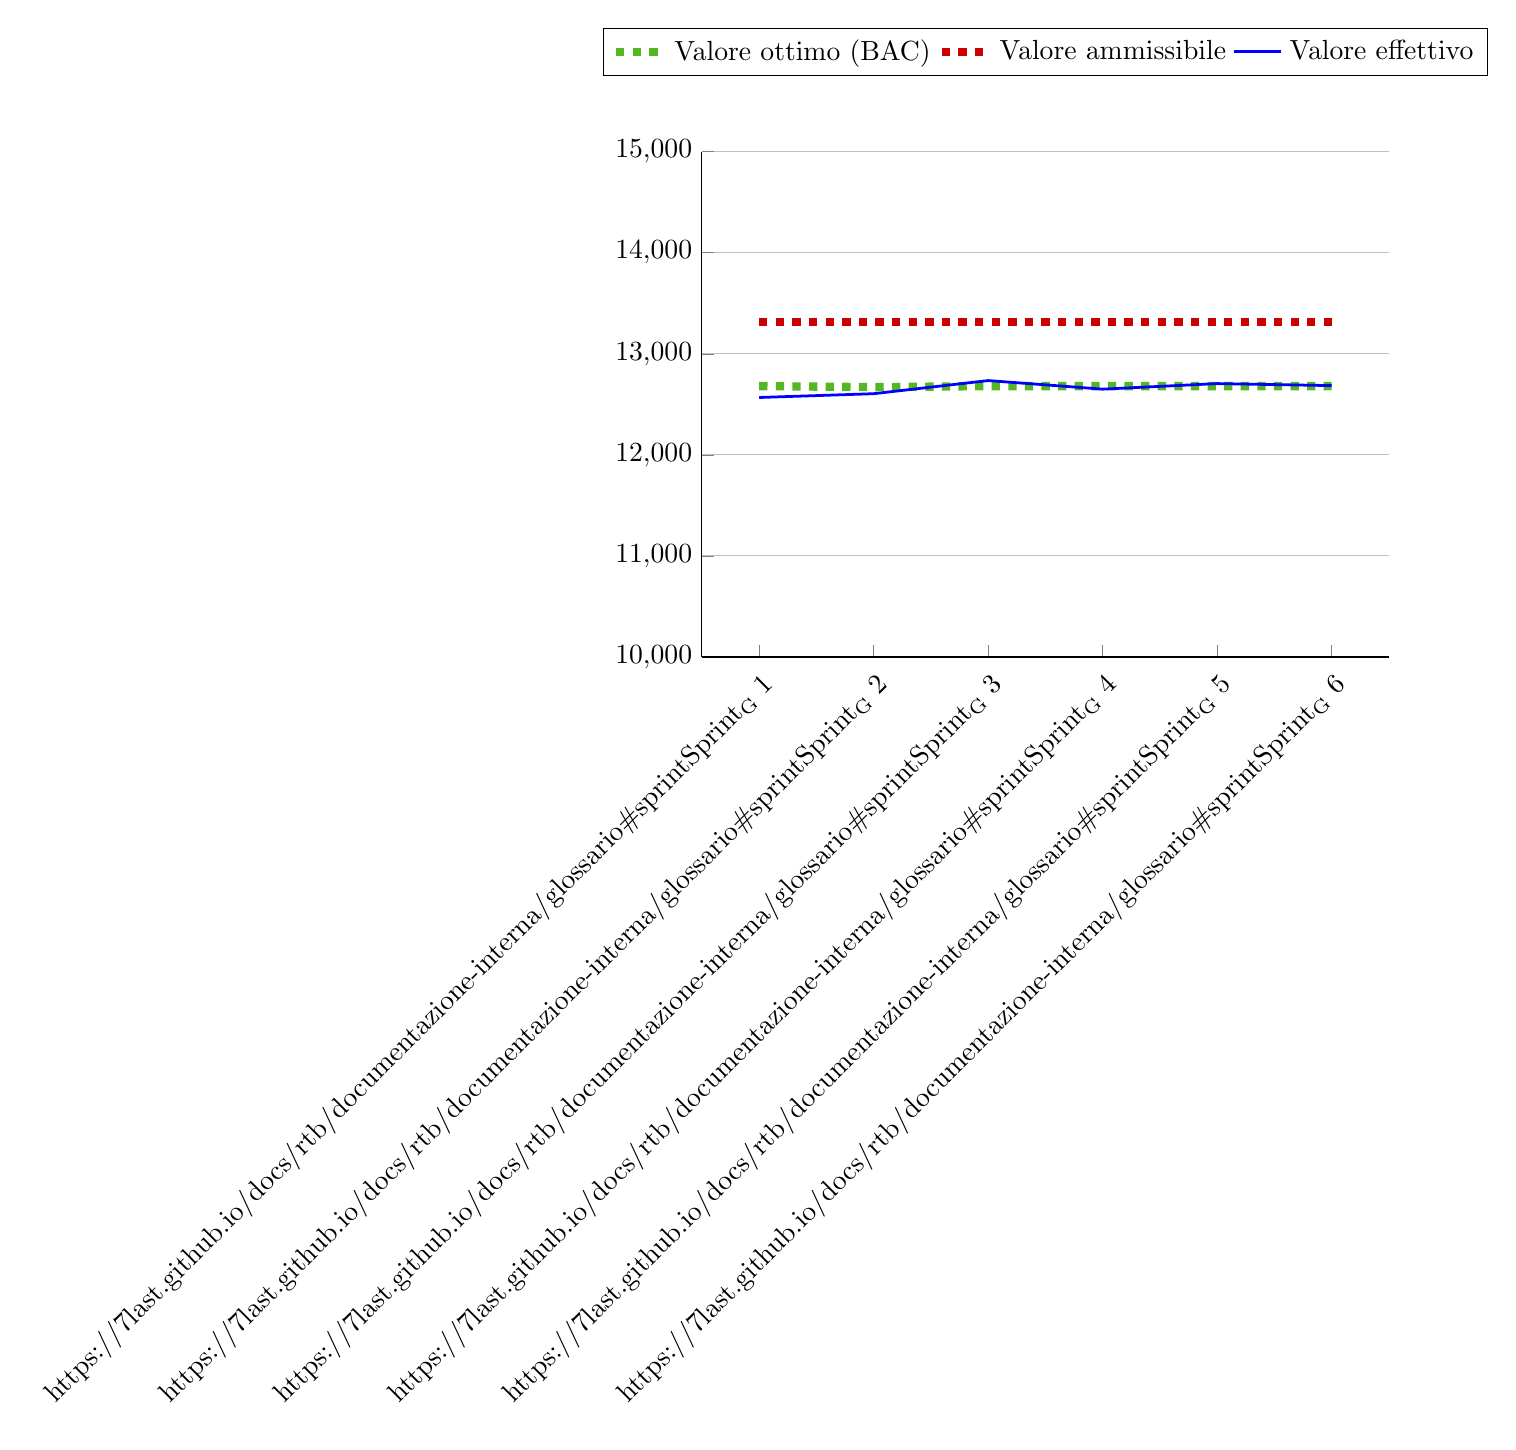
\begin{tikzpicture}
        \begin{axis}[
            width  = 0.85*\textwidth,
            height = 8cm,
            ymajorgrids = true,
            symbolic x coords={\href{https://7last.github.io/docs/rtb/documentazione-interna/glossario\#sprint}{Sprint\textsubscript{G}} 1, \href{https://7last.github.io/docs/rtb/documentazione-interna/glossario\#sprint}{Sprint\textsubscript{G}} 2, \href{https://7last.github.io/docs/rtb/documentazione-interna/glossario\#sprint}{Sprint\textsubscript{G}} 3, \href{https://7last.github.io/docs/rtb/documentazione-interna/glossario\#sprint}{Sprint\textsubscript{G}} 4, \href{https://7last.github.io/docs/rtb/documentazione-interna/glossario\#sprint}{Sprint\textsubscript{G}} 5, \href{https://7last.github.io/docs/rtb/documentazione-interna/glossario\#sprint}{Sprint\textsubscript{G}} 6},
            xtick = data,
            ytick = {10000, 11000, 12000, 13000, 14000, 15000},
            ymin=10000, ymax=15000,
            axis lines*=left,
            legend cell align=left,
            legend style={
                at={(0.5,1.15)},
                anchor=south,
                column sep=0.1ex,
                legend columns=3
            },
            xticklabel style={rotate=45, anchor=north east, yshift=0ex, xshift=0ex},
            scaled y ticks = false,
            yticklabel style={/pgf/number format/fixed}
        ]
            \addplot[color=opt, style={dashed, line width=3pt}, mark=none] coordinates {(\href{https://7last.github.io/docs/rtb/documentazione-interna/glossario\#sprint}{Sprint\textsubscript{G}} 1, 12680) (\href{https://7last.github.io/docs/rtb/documentazione-interna/glossario\#sprint}{Sprint\textsubscript{G}} 2, 12670) (\href{https://7last.github.io/docs/rtb/documentazione-interna/glossario\#sprint}{Sprint\textsubscript{G}} 3, 12680) (\href{https://7last.github.io/docs/rtb/documentazione-interna/glossario\#sprint}{Sprint\textsubscript{G}} 4, 12680) (\href{https://7last.github.io/docs/rtb/documentazione-interna/glossario\#sprint}{Sprint\textsubscript{G}} 5, 12680) (\href{https://7last.github.io/docs/rtb/documentazione-interna/glossario\#sprint}{Sprint\textsubscript{G}} 6, 12680)}; % ottimo = BAC
            \addplot[color=amm, style={dashed, line width=3pt}, mark=none] coordinates {(\href{https://7last.github.io/docs/rtb/documentazione-interna/glossario\#sprint}{Sprint\textsubscript{G}} 1, 13314) (\href{https://7last.github.io/docs/rtb/documentazione-interna/glossario\#sprint}{Sprint\textsubscript{G}} 2, 13314) (\href{https://7last.github.io/docs/rtb/documentazione-interna/glossario\#sprint}{Sprint\textsubscript{G}} 3, 13314) (\href{https://7last.github.io/docs/rtb/documentazione-interna/glossario\#sprint}{Sprint\textsubscript{G}} 4, 13314) (\href{https://7last.github.io/docs/rtb/documentazione-interna/glossario\#sprint}{Sprint\textsubscript{G}} 5, 13314) (\href{https://7last.github.io/docs/rtb/documentazione-interna/glossario\#sprint}{Sprint\textsubscript{G}} 6, 13314)}; % ammissibile = BAC + 5%
            \addplot[color=blue, style={line width=1pt}, mark=none] coordinates {(\href{https://7last.github.io/docs/rtb/documentazione-interna/glossario\#sprint}{Sprint\textsubscript{G}} 1, 12567.5) (\href{https://7last.github.io/docs/rtb/documentazione-interna/glossario\#sprint}{Sprint\textsubscript{G}} 2, 12605) (\href{https://7last.github.io/docs/rtb/documentazione-interna/glossario\#sprint}{Sprint\textsubscript{G}} 3, 12735) (\href{https://7last.github.io/docs/rtb/documentazione-interna/glossario\#sprint}{Sprint\textsubscript{G}} 4, 12650) (\href{https://7last.github.io/docs/rtb/documentazione-interna/glossario\#sprint}{Sprint\textsubscript{G}} 5, 12705) (\href{https://7last.github.io/docs/rtb/documentazione-interna/glossario\#sprint}{Sprint\textsubscript{G}} 6, 12685)}; % EAC
            \legend{Valore ottimo (BAC), Valore ammissibile, Valore effettivo}
        \end{axis}
    \end{tikzpicture}
    \caption{Proiezione dell'EAC}
\end{figure*}
%--------- FINE GRAFICO -----------%
\subsubsection*{\href{https://7last.github.io/docs/rtb/documentazione-interna/glossario\#requirements-and-technology-baseline}{RTB\textsubscript{G}}}
Osservando il grafico si può notare come l'EAC sia quasi sovrapposto al BAC durante i periodi di progetto analizzati fino ad ora. Questa situazione riflette come \textit{7Last} abbia attuato una gestione efficace sia dei costi che delle tempistiche durante i periodi analizzati fino ad ora.

%TODO mettere considerazioni finali \href{https://7last.github.io/docs/rtb/documentazione-interna/glossario\#product-baseline}{PB\textsubscript{G}}
% \newpage

% \subsection{Qualità del processo di Analisi dei requisiti}
% \subsubsection{11M-PRO - Percentuale Requisiti Obbligatori}
% %--------- GRAFICO -----------%
% \begin{figure*}[!h]
%     \centering
%     \begin{tikzpicture}
%         \begin{axis}[
%             width  = 0.85*\textwidth,
%             height = 8cm,
%             ymajorgrids = true,
%             symbolic x coords={\href{https://7last.github.io/docs/rtb/documentazione-interna/glossario\#sprint}{Sprint\textsubscript{G}} 1, \href{https://7last.github.io/docs/rtb/documentazione-interna/glossario\#sprint}{Sprint\textsubscript{G}} 2, \href{https://7last.github.io/docs/rtb/documentazione-interna/glossario\#sprint}{Sprint\textsubscript{G}} 3, \href{https://7last.github.io/docs/rtb/documentazione-interna/glossario\#sprint}{Sprint\textsubscript{G}} 4},
%             xtick = data,
%             ytick = {0, 25, 50, 75, 100},
%             ymin=0, ymax=100,
%             axis lines*=left,
%             legend cell align=left,
%             legend style={
%                 at={(0.5,1.15)},
%                 anchor=south,
%                 column sep=0.1ex,
%                 legend columns=3
%             },
%             xticklabel style={rotate=45, anchor=north east, yshift=0ex, xshift=0ex}
%             ]
%             \addplot[color=opt, style={dashed, line width=3pt}, mark=none] coordinates {(\href{https://7last.github.io/docs/rtb/documentazione-interna/glossario\#sprint}{Sprint\textsubscript{G}} 1, 100) (\href{https://7last.github.io/docs/rtb/documentazione-interna/glossario\#sprint}{Sprint\textsubscript{G}} 2, 100) (\href{https://7last.github.io/docs/rtb/documentazione-interna/glossario\#sprint}{Sprint\textsubscript{G}} 3, 100) (\href{https://7last.github.io/docs/rtb/documentazione-interna/glossario\#sprint}{Sprint\textsubscript{G}} 4, 100)};
%             \addplot[color=blue, style={line width=1pt}, mark=none] coordinates {(\href{https://7last.github.io/docs/rtb/documentazione-interna/glossario\#sprint}{Sprint\textsubscript{G}} 1, 25) (\href{https://7last.github.io/docs/rtb/documentazione-interna/glossario\#sprint}{Sprint\textsubscript{G}} 2, 48) (\href{https://7last.github.io/docs/rtb/documentazione-interna/glossario\#sprint}{Sprint\textsubscript{G}} 3, 52) (\href{https://7last.github.io/docs/rtb/documentazione-interna/glossario\#sprint}{Sprint\textsubscript{G}} 4, 64)};
%             \legend{Valore ottimo ed ammissibile, Valore effettivo}
%         \end{axis}
%     \end{tikzpicture}
%     %44 requisiti obbligatori, 11 implementati nel primo \href{https://7last.github.io/docs/rtb/documentazione-interna/glossario\#sprint}{sprint\textsubscript{G}}, 21 nel secondo e 24 nel terzo, 28 nel quarto
%     \caption{Percentuale di copertura dei requisiti obbligatori}
% \end{figure*}
% %--------- FINE GRAFICO -----------%
% \subsubsection*{\href{https://7last.github.io/docs/rtb/documentazione-interna/glossario\#requirements-and-technology-baseline}{RTB\textsubscript{G}}}

% %TODO mettere considerazioni finali \href{https://7last.github.io/docs/rtb/documentazione-interna/glossario\#product-baseline}{PB\textsubscript{G}}
% \newpage
% \subsubsection{12M-PRD - Percentuale Requisiti Desiderabili}
% %--------- GRAFICO -----------%
% \begin{figure*}[!h]
%     \centering
%     \begin{tikzpicture}
%         \begin{axis}[
%             width  = 0.85*\textwidth,
%             height = 8cm,
%             ymajorgrids = true,
%             symbolic x coords={\href{https://7last.github.io/docs/rtb/documentazione-interna/glossario\#sprint}{Sprint\textsubscript{G}} 1, \href{https://7last.github.io/docs/rtb/documentazione-interna/glossario\#sprint}{Sprint\textsubscript{G}} 2, \href{https://7last.github.io/docs/rtb/documentazione-interna/glossario\#sprint}{Sprint\textsubscript{G}} 3, \href{https://7last.github.io/docs/rtb/documentazione-interna/glossario\#sprint}{Sprint\textsubscript{G}} 4},
%             xtick = data,
%             ytick = {0, 25, 50, 75, 100},
%             ymin=0, ymax=100,
%             axis lines*=left,
%             legend cell align=left,
%             legend style={
%                 at={(0.5,1.15)},
%                 anchor=south,
%                 column sep=0.1ex,
%                 legend columns=3
%             },
%             xticklabel style={rotate=45, anchor=north east, yshift=0ex, xshift=0ex}
%             ]
%             \addplot[color=opt, style={dashed, line width=3pt}, mark=none] coordinates {(\href{https://7last.github.io/docs/rtb/documentazione-interna/glossario\#sprint}{Sprint\textsubscript{G}} 1, 100) (\href{https://7last.github.io/docs/rtb/documentazione-interna/glossario\#sprint}{Sprint\textsubscript{G}} 2, 100) (\href{https://7last.github.io/docs/rtb/documentazione-interna/glossario\#sprint}{Sprint\textsubscript{G}} 3, 100) (\href{https://7last.github.io/docs/rtb/documentazione-interna/glossario\#sprint}{Sprint\textsubscript{G}} 4, 100)};
%             \addplot[color=amm, style={dashed, line width=3pt}, mark=none] coordinates {(\href{https://7last.github.io/docs/rtb/documentazione-interna/glossario\#sprint}{Sprint\textsubscript{G}} 1, 35) (\href{https://7last.github.io/docs/rtb/documentazione-interna/glossario\#sprint}{Sprint\textsubscript{G}} 2, 35) (\href{https://7last.github.io/docs/rtb/documentazione-interna/glossario\#sprint}{Sprint\textsubscript{G}} 3, 35) (\href{https://7last.github.io/docs/rtb/documentazione-interna/glossario\#sprint}{Sprint\textsubscript{G}} 4, 35)};
%             \addplot[color=blue, style={line width=1pt}, mark=none] coordinates {(\href{https://7last.github.io/docs/rtb/documentazione-interna/glossario\#sprint}{Sprint\textsubscript{G}} 1, 0) (\href{https://7last.github.io/docs/rtb/documentazione-interna/glossario\#sprint}{Sprint\textsubscript{G}} 2, 20) (\href{https://7last.github.io/docs/rtb/documentazione-interna/glossario\#sprint}{Sprint\textsubscript{G}} 3, 40) (\href{https://7last.github.io/docs/rtb/documentazione-interna/glossario\#sprint}{Sprint\textsubscript{G}} 4, 60)};
%             \legend{Valore ottimo, Valore ammissibile, Valore effettivo}
%         \end{axis}
%     \end{tikzpicture}
%     \caption{Percentuale di copertura dei requisiti desiderabili}
% \end{figure*}
% %5 requisiti desiderabili; 0 nel primo \href{https://7last.github.io/docs/rtb/documentazione-interna/glossario\#sprint}{sprint\textsubscript{G}}, 1 nel secondo,1 nel terzo, 1 nel quarto
% %--------- FINE GRAFICO -----------%
% %\href{https://7last.github.io/docs/rtb/documentazione-interna/glossario\#requirements-and-technology-baseline}{\textbf{RTB}\textsubscript{G}} \\
% % TODO considerazioni finali per \href{https://7last.github.io/docs/rtb/documentazione-interna/glossario\#requirements-and-technology-baseline}{RTB\textsubscript{G}} \\
% %\href{https://7last.github.io/docs/rtb/documentazione-interna/glossario\#product-baseline}{\textbf{PB}\textsubscript{G}} \\
% % TODO considerazioni finali per \href{https://7last.github.io/docs/rtb/documentazione-interna/glossario\#product-baseline}{PB\textsubscript{G}}

% \newpage
% \subsubsection{13M-PRO - Percentuale Requisiti Opzionali}
% %--------- GRAFICO -----------%
% \begin{figure*}[!h]
%     \centering
%     \begin{tikzpicture}
%         \begin{axis}[
%             width  = 0.85*\textwidth,
%             height = 8cm,
%             ymajorgrids = true,
%             symbolic x coords={\href{https://7last.github.io/docs/rtb/documentazione-interna/glossario\#sprint}{Sprint\textsubscript{G}} 1, \href{https://7last.github.io/docs/rtb/documentazione-interna/glossario\#sprint}{Sprint\textsubscript{G}} 2, \href{https://7last.github.io/docs/rtb/documentazione-interna/glossario\#sprint}{Sprint\textsubscript{G}} 3, \href{https://7last.github.io/docs/rtb/documentazione-interna/glossario\#sprint}{Sprint\textsubscript{G}} 4},
%             xtick = data,
%             ytick = {0, 25, 50, 75, 100},
%             ymin=0, ymax=100,
%             axis lines*=left,
%             legend cell align=left,
%             legend style={
%                 at={(0.5,1.15)},
%                 anchor=south,
%                 column sep=0.1ex,
%                 legend columns=3
%             },
%             xticklabel style={rotate=45, anchor=north east, yshift=0ex, xshift=0ex}
%             ]
%             \addplot[color=opt, style={dashed, line width=3pt}, mark=none] coordinates {(\href{https://7last.github.io/docs/rtb/documentazione-interna/glossario\#sprint}{Sprint\textsubscript{G}} 1, 100) (\href{https://7last.github.io/docs/rtb/documentazione-interna/glossario\#sprint}{Sprint\textsubscript{G}} 2, 100) (\href{https://7last.github.io/docs/rtb/documentazione-interna/glossario\#sprint}{Sprint\textsubscript{G}} 3, 100) (\href{https://7last.github.io/docs/rtb/documentazione-interna/glossario\#sprint}{Sprint\textsubscript{G}} 4, 100)};
%             \addplot[color=amm, style={dashed, line width=3pt}, mark=none] coordinates {(\href{https://7last.github.io/docs/rtb/documentazione-interna/glossario\#sprint}{Sprint\textsubscript{G}} 1, 0) (\href{https://7last.github.io/docs/rtb/documentazione-interna/glossario\#sprint}{Sprint\textsubscript{G}} 2, 0) (\href{https://7last.github.io/docs/rtb/documentazione-interna/glossario\#sprint}{Sprint\textsubscript{G}} 3, 0) (\href{https://7last.github.io/docs/rtb/documentazione-interna/glossario\#sprint}{Sprint\textsubscript{G}} 4, 0)};
%             \addplot[color=blue, style={line width=1pt}, mark=none] coordinates {(\href{https://7last.github.io/docs/rtb/documentazione-interna/glossario\#sprint}{Sprint\textsubscript{G}} 1, 0) (\href{https://7last.github.io/docs/rtb/documentazione-interna/glossario\#sprint}{Sprint\textsubscript{G}} 2, 0) (\href{https://7last.github.io/docs/rtb/documentazione-interna/glossario\#sprint}{Sprint\textsubscript{G}} 3, 0) (\href{https://7last.github.io/docs/rtb/documentazione-interna/glossario\#sprint}{Sprint\textsubscript{G}} 4, 33)};
%             \legend{Valore ottimo, Valore ammissibile, Valore effettivo}
%         \end{axis}
%     \end{tikzpicture}
%     \caption{Percentuale di copertura dei requisiti opzionali}
%     %3 requisiti opzionali, 0 primo \href{https://7last.github.io/docs/rtb/documentazione-interna/glossario\#sprint}{sprint\textsubscript{G}}, 0 secondo \href{https://7last.github.io/docs/rtb/documentazione-interna/glossario\#sprint}{sprint\textsubscript{G}}, 0 terzo \href{https://7last.github.io/docs/rtb/documentazione-interna/glossario\#sprint}{sprint\textsubscript{G}} 1 quarto \href{https://7last.github.io/docs/rtb/documentazione-interna/glossario\#sprint}{sprint\textsubscript{G}}
% \end{figure*}


%--------- FINE GRAFICO -----------%
%\href{https://7last.github.io/docs/rtb/documentazione-interna/glossario\#requirements-and-technology-baseline}{\textbf{RTB}\textsubscript{G}} \\
% TODO considerazioni finali per \href{https://7last.github.io/docs/rtb/documentazione-interna/glossario\#requirements-and-technology-baseline}{RTB\textsubscript{G}} \\
%\href{https://7last.github.io/docs/rtb/documentazione-interna/glossario\#product-baseline}{\textbf{PB}\textsubscript{G}} \\
% TODO considerazioni finali per \href{https://7last.github.io/docs/rtb/documentazione-interna/glossario\#product-baseline}{PB\textsubscript{G}}



\newpage
\subsection{Qualità del processo di Documentazione}
\subsubsection{19M-IG - Indice Gulpease}
%--------- GRAFICO -----------%
\begin{figure*}[!h]
    \centering
    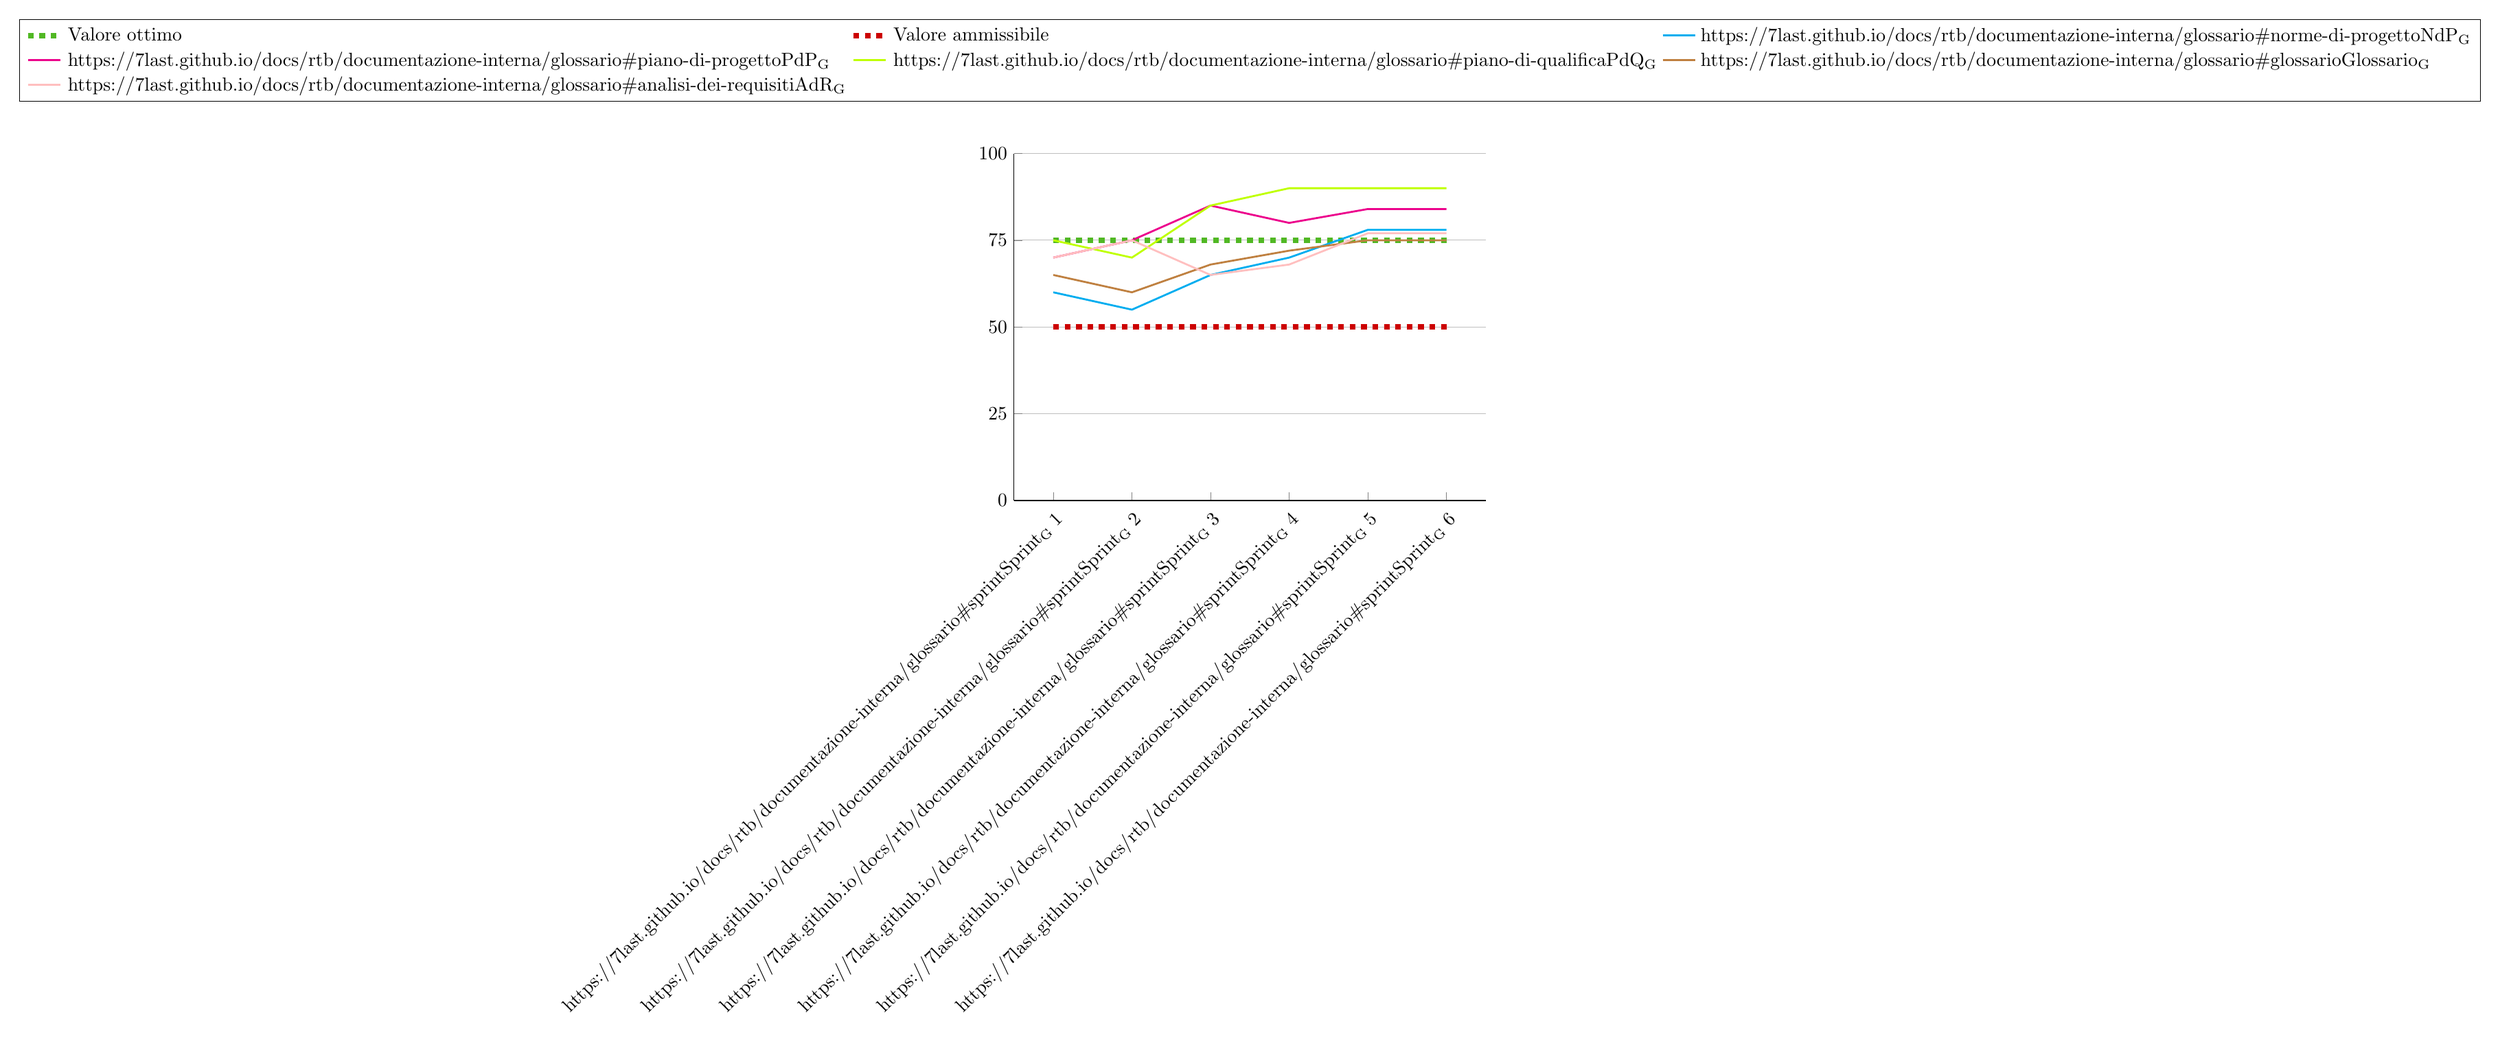
\begin{tikzpicture}
        \begin{axis}[
            width  = 0.85*\textwidth,
            height = 8cm,
            ymajorgrids = true,
            symbolic x coords={\href{https://7last.github.io/docs/rtb/documentazione-interna/glossario\#sprint}{Sprint\textsubscript{G}} 1, \href{https://7last.github.io/docs/rtb/documentazione-interna/glossario\#sprint}{Sprint\textsubscript{G}} 2, \href{https://7last.github.io/docs/rtb/documentazione-interna/glossario\#sprint}{Sprint\textsubscript{G}} 3, \href{https://7last.github.io/docs/rtb/documentazione-interna/glossario\#sprint}{Sprint\textsubscript{G}} 4, \href{https://7last.github.io/docs/rtb/documentazione-interna/glossario\#sprint}{Sprint\textsubscript{G}} 5, \href{https://7last.github.io/docs/rtb/documentazione-interna/glossario\#sprint}{Sprint\textsubscript{G}} 6},
            xtick = data,
            ytick = {0, 25, 50, 75, 100},
            ymin=0, ymax=100,
            axis lines*=left,
            legend cell align=left,
            legend style={
                at={(0.5,1.15)},
                anchor=south,
                column sep=0.1ex,
                legend columns=3
            },
            xticklabel style={rotate=45, anchor=north east, yshift=0ex, xshift=0ex}
        ]
            \addplot[color=opt, style={dashed, line width=3pt}, mark=none] coordinates {(\href{https://7last.github.io/docs/rtb/documentazione-interna/glossario\#sprint}{Sprint\textsubscript{G}} 1, 75) (\href{https://7last.github.io/docs/rtb/documentazione-interna/glossario\#sprint}{Sprint\textsubscript{G}} 2, 75) (\href{https://7last.github.io/docs/rtb/documentazione-interna/glossario\#sprint}{Sprint\textsubscript{G}} 3, 75) (\href{https://7last.github.io/docs/rtb/documentazione-interna/glossario\#sprint}{Sprint\textsubscript{G}} 4, 75) (\href{https://7last.github.io/docs/rtb/documentazione-interna/glossario\#sprint}{Sprint\textsubscript{G}} 5, 75) (\href{https://7last.github.io/docs/rtb/documentazione-interna/glossario\#sprint}{Sprint\textsubscript{G}} 6, 75)}; % ottimo = 75
            \addplot[color=amm, style={dashed, line width=3pt}, mark=none] coordinates {(\href{https://7last.github.io/docs/rtb/documentazione-interna/glossario\#sprint}{Sprint\textsubscript{G}} 1, 50) (\href{https://7last.github.io/docs/rtb/documentazione-interna/glossario\#sprint}{Sprint\textsubscript{G}} 2, 50) (\href{https://7last.github.io/docs/rtb/documentazione-interna/glossario\#sprint}{Sprint\textsubscript{G}} 3, 50) (\href{https://7last.github.io/docs/rtb/documentazione-interna/glossario\#sprint}{Sprint\textsubscript{G}} 4, 50) (\href{https://7last.github.io/docs/rtb/documentazione-interna/glossario\#sprint}{Sprint\textsubscript{G}} 5, 50) (\href{https://7last.github.io/docs/rtb/documentazione-interna/glossario\#sprint}{Sprint\textsubscript{G}} 6, 50)}; % ammissibile = 50
            \addplot[color=cyan, style={line width=1pt}, mark=none] coordinates {(\href{https://7last.github.io/docs/rtb/documentazione-interna/glossario\#sprint}{Sprint\textsubscript{G}} 1, 60) (\href{https://7last.github.io/docs/rtb/documentazione-interna/glossario\#sprint}{Sprint\textsubscript{G}} 2, 55) (\href{https://7last.github.io/docs/rtb/documentazione-interna/glossario\#sprint}{Sprint\textsubscript{G}} 3, 65) (\href{https://7last.github.io/docs/rtb/documentazione-interna/glossario\#sprint}{Sprint\textsubscript{G}} 4, 70) (\href{https://7last.github.io/docs/rtb/documentazione-interna/glossario\#sprint}{Sprint\textsubscript{G}} 5, 78) (\href{https://7last.github.io/docs/rtb/documentazione-interna/glossario\#sprint}{Sprint\textsubscript{G}} 6, 78)}; % \href{https://7last.github.io/docs/rtb/documentazione-interna/glossario\#norme-di-progetto}{NdP\textsubscript{G}}
            \addplot[color=magenta, style={line width=1pt}, mark=none] coordinates {(\href{https://7last.github.io/docs/rtb/documentazione-interna/glossario\#sprint}{Sprint\textsubscript{G}} 1, 70) (\href{https://7last.github.io/docs/rtb/documentazione-interna/glossario\#sprint}{Sprint\textsubscript{G}} 2, 75) (\href{https://7last.github.io/docs/rtb/documentazione-interna/glossario\#sprint}{Sprint\textsubscript{G}} 3, 85) (\href{https://7last.github.io/docs/rtb/documentazione-interna/glossario\#sprint}{Sprint\textsubscript{G}} 4, 80) (\href{https://7last.github.io/docs/rtb/documentazione-interna/glossario\#sprint}{Sprint\textsubscript{G}} 5, 84) (\href{https://7last.github.io/docs/rtb/documentazione-interna/glossario\#sprint}{Sprint\textsubscript{G}} 6, 84)}; % \href{https://7last.github.io/docs/rtb/documentazione-interna/glossario\#piano-di-progetto}{PdP\textsubscript{G}}
            \addplot[color=lime, style={line width=1pt}, mark=none] coordinates {(\href{https://7last.github.io/docs/rtb/documentazione-interna/glossario\#sprint}{Sprint\textsubscript{G}} 1, 75) (\href{https://7last.github.io/docs/rtb/documentazione-interna/glossario\#sprint}{Sprint\textsubscript{G}} 2, 70) (\href{https://7last.github.io/docs/rtb/documentazione-interna/glossario\#sprint}{Sprint\textsubscript{G}} 3, 85) (\href{https://7last.github.io/docs/rtb/documentazione-interna/glossario\#sprint}{Sprint\textsubscript{G}} 4, 90) (\href{https://7last.github.io/docs/rtb/documentazione-interna/glossario\#sprint}{Sprint\textsubscript{G}} 5, 90) (\href{https://7last.github.io/docs/rtb/documentazione-interna/glossario\#sprint}{Sprint\textsubscript{G}} 6, 90)}; % \href{https://7last.github.io/docs/rtb/documentazione-interna/glossario\#piano-di-qualifica}{PdQ\textsubscript{G}}
            \addplot[color=brown, style={line width=1pt}, mark=none] coordinates {(\href{https://7last.github.io/docs/rtb/documentazione-interna/glossario\#sprint}{Sprint\textsubscript{G}} 1, 65) (\href{https://7last.github.io/docs/rtb/documentazione-interna/glossario\#sprint}{Sprint\textsubscript{G}} 2, 60) (\href{https://7last.github.io/docs/rtb/documentazione-interna/glossario\#sprint}{Sprint\textsubscript{G}} 3, 68) (\href{https://7last.github.io/docs/rtb/documentazione-interna/glossario\#sprint}{Sprint\textsubscript{G}} 4, 72) (\href{https://7last.github.io/docs/rtb/documentazione-interna/glossario\#sprint}{Sprint\textsubscript{G}} 5, 75) (\href{https://7last.github.io/docs/rtb/documentazione-interna/glossario\#sprint}{Sprint\textsubscript{G}} 6, 75)}; % Glo
            \addplot[color=pink, style={line width=1pt}, mark=none] coordinates {(\href{https://7last.github.io/docs/rtb/documentazione-interna/glossario\#sprint}{Sprint\textsubscript{G}} 1, 70) (\href{https://7last.github.io/docs/rtb/documentazione-interna/glossario\#sprint}{Sprint\textsubscript{G}} 2, 75) (\href{https://7last.github.io/docs/rtb/documentazione-interna/glossario\#sprint}{Sprint\textsubscript{G}} 3, 65) (\href{https://7last.github.io/docs/rtb/documentazione-interna/glossario\#sprint}{Sprint\textsubscript{G}} 4, 68) (\href{https://7last.github.io/docs/rtb/documentazione-interna/glossario\#sprint}{Sprint\textsubscript{G}} 5, 77) (\href{https://7last.github.io/docs/rtb/documentazione-interna/glossario\#sprint}{Sprint\textsubscript{G}} 6, 77)}; % \href{https://7last.github.io/docs/rtb/documentazione-interna/glossario\#analisi-dei-requisiti}{AdR\textsubscript{G}}
            \addplot[color=violet, style={line width=1pt}, mark=none] coordinates {}; % MU
            \addplot[color=yellow, style={line width=1pt}, mark=none] coordinates {}; % ST
            \legend{Valore ottimo, Valore ammissibile, \href{https://7last.github.io/docs/rtb/documentazione-interna/glossario\#norme-di-progetto}{NdP\textsubscript{G}}, \href{https://7last.github.io/docs/rtb/documentazione-interna/glossario\#piano-di-progetto}{PdP\textsubscript{G}}, \href{https://7last.github.io/docs/rtb/documentazione-interna/glossario\#piano-di-qualifica}{PdQ\textsubscript{G}}, \href{https://7last.github.io/docs/rtb/documentazione-interna/glossario\#glossario}{Glossario\textsubscript{G}}, \href{https://7last.github.io/docs/rtb/documentazione-interna/glossario\#analisi-dei-requisiti}{AdR\textsubscript{G}}, MU, ST}
        \end{axis}
    \end{tikzpicture}
    \caption{Andamento indice di Gulpease per ciascun documento}
\end{figure*}
%--------- FINE GRAFICO -----------%
\subsubsection*{\href{https://7last.github.io/docs/rtb/documentazione-interna/glossario\#requirements-and-technology-baseline}{RTB\textsubscript{G}}}
Visionando il grafico si può notare una tendenza generale di crescita, eccetto per alcuni documenti. L'indice relativamente basso rispetto agli altri documenti rappresenta il \href{https://7last.github.io/docs/rtb/documentazione-interna/glossario\#glossario}{glossario\textsubscript{G}}, il quale contiene descrizioni di natura tecnica che possono influire negativamente sull'indice di Gulpease.

%TODO mettere considerazioni finali \href{https://7last.github.io/docs/rtb/documentazione-interna/glossario\#product-baseline}{PB\textsubscript{G}}
\newpage
\subsubsection{20M-CO - Correttezza Ortografica}
%--------- GRAFICO -----------%
\begin{figure*}[!h]
    \centering
    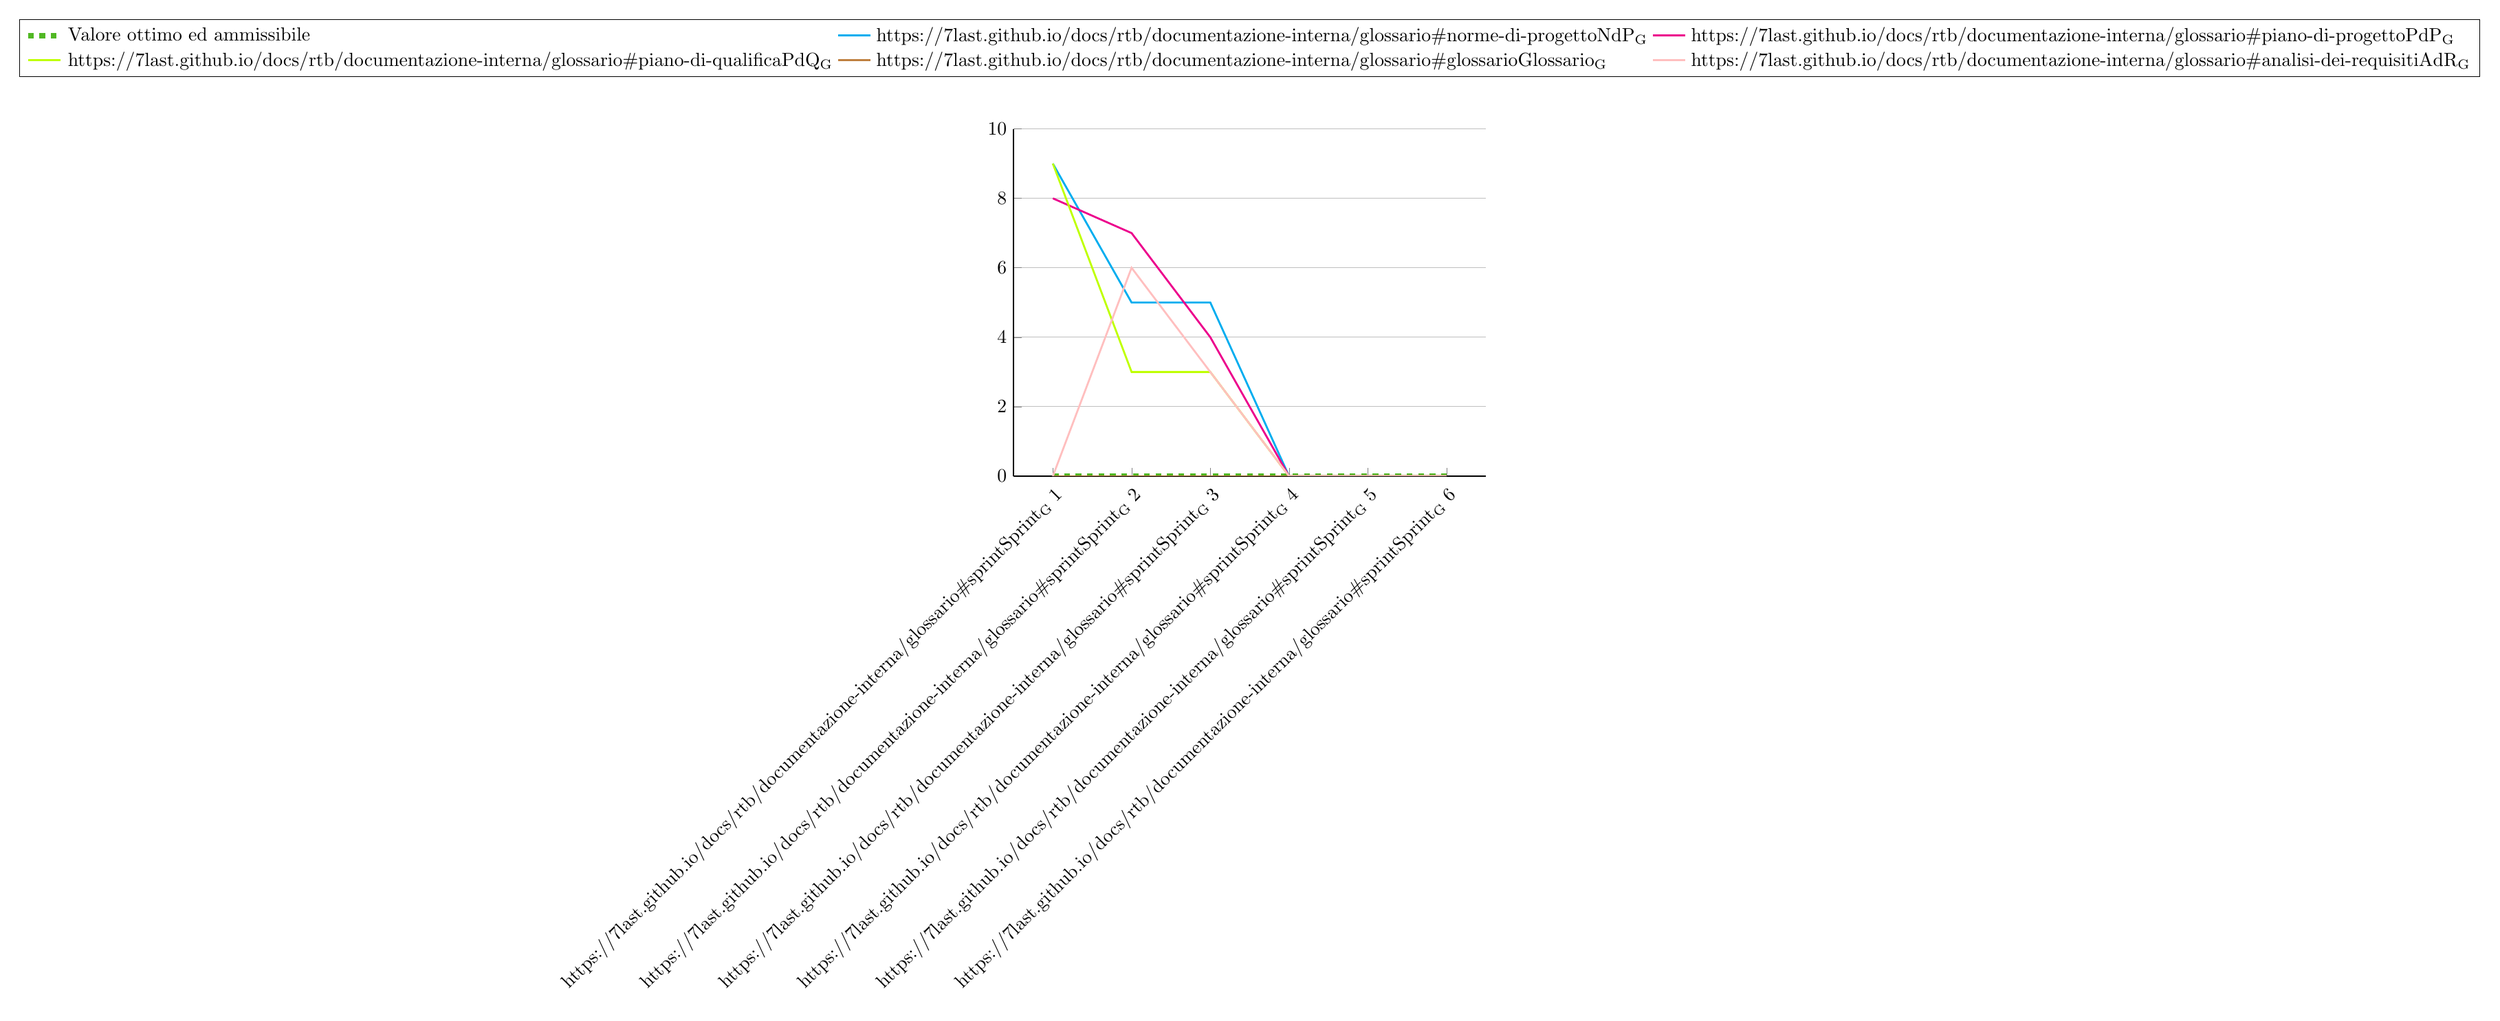
\begin{tikzpicture}
        \begin{axis}[
            width  = 0.85*\textwidth,
            height = 8cm,
            ymajorgrids = true,
            symbolic x coords={\href{https://7last.github.io/docs/rtb/documentazione-interna/glossario\#sprint}{Sprint\textsubscript{G}} 1, \href{https://7last.github.io/docs/rtb/documentazione-interna/glossario\#sprint}{Sprint\textsubscript{G}} 2, \href{https://7last.github.io/docs/rtb/documentazione-interna/glossario\#sprint}{Sprint\textsubscript{G}} 3, \href{https://7last.github.io/docs/rtb/documentazione-interna/glossario\#sprint}{Sprint\textsubscript{G}} 4, \href{https://7last.github.io/docs/rtb/documentazione-interna/glossario\#sprint}{Sprint\textsubscript{G}} 5, \href{https://7last.github.io/docs/rtb/documentazione-interna/glossario\#sprint}{Sprint\textsubscript{G}} 6},
            xtick = data,
            ymin=0, ymax=10,
            axis lines*=left,
            legend cell align=left,
            legend style={
                at={(0.5,1.15)},
                anchor=south,
                column sep=0.1ex,
                legend columns=3
            },
            xticklabel style={rotate=45, anchor=north east, yshift=0ex, xshift=0ex}
        ]
            \addplot[color=opt, style={dashed, line width=3pt}, mark=none] coordinates {(\href{https://7last.github.io/docs/rtb/documentazione-interna/glossario\#sprint}{Sprint\textsubscript{G}} 1, 0) (\href{https://7last.github.io/docs/rtb/documentazione-interna/glossario\#sprint}{Sprint\textsubscript{G}} 2, 0) (\href{https://7last.github.io/docs/rtb/documentazione-interna/glossario\#sprint}{Sprint\textsubscript{G}} 3, 0) (\href{https://7last.github.io/docs/rtb/documentazione-interna/glossario\#sprint}{Sprint\textsubscript{G}} 4, 0) (\href{https://7last.github.io/docs/rtb/documentazione-interna/glossario\#sprint}{Sprint\textsubscript{G}} 5, 0) (\href{https://7last.github.io/docs/rtb/documentazione-interna/glossario\#sprint}{Sprint\textsubscript{G}} 6, 0)}; % ottimo e ammissibile = 0
            \addplot[color=cyan, style={line width=1pt}, mark=none] coordinates {(\href{https://7last.github.io/docs/rtb/documentazione-interna/glossario\#sprint}{Sprint\textsubscript{G}} 1, 9) (\href{https://7last.github.io/docs/rtb/documentazione-interna/glossario\#sprint}{Sprint\textsubscript{G}} 2, 5) (\href{https://7last.github.io/docs/rtb/documentazione-interna/glossario\#sprint}{Sprint\textsubscript{G}} 3, 5) (\href{https://7last.github.io/docs/rtb/documentazione-interna/glossario\#sprint}{Sprint\textsubscript{G}} 4, 0) (\href{https://7last.github.io/docs/rtb/documentazione-interna/glossario\#sprint}{Sprint\textsubscript{G}} 5, 0) (\href{https://7last.github.io/docs/rtb/documentazione-interna/glossario\#sprint}{Sprint\textsubscript{G}} 6, 0)}; % \href{https://7last.github.io/docs/rtb/documentazione-interna/glossario\#norme-di-progetto}{NdP\textsubscript{G}}
            \addplot[color=magenta, style={line width=1pt}, mark=none] coordinates {(\href{https://7last.github.io/docs/rtb/documentazione-interna/glossario\#sprint}{Sprint\textsubscript{G}} 1, 8) (\href{https://7last.github.io/docs/rtb/documentazione-interna/glossario\#sprint}{Sprint\textsubscript{G}} 2, 7) (\href{https://7last.github.io/docs/rtb/documentazione-interna/glossario\#sprint}{Sprint\textsubscript{G}} 3, 4) (\href{https://7last.github.io/docs/rtb/documentazione-interna/glossario\#sprint}{Sprint\textsubscript{G}} 4, 0) (\href{https://7last.github.io/docs/rtb/documentazione-interna/glossario\#sprint}{Sprint\textsubscript{G}} 5, 0) (\href{https://7last.github.io/docs/rtb/documentazione-interna/glossario\#sprint}{Sprint\textsubscript{G}} 6, 0)}; % \href{https://7last.github.io/docs/rtb/documentazione-interna/glossario\#piano-di-progetto}{PdP\textsubscript{G}}
            \addplot[color=lime, style={line width=1pt}, mark=none] coordinates {(\href{https://7last.github.io/docs/rtb/documentazione-interna/glossario\#sprint}{Sprint\textsubscript{G}} 1, 9) (\href{https://7last.github.io/docs/rtb/documentazione-interna/glossario\#sprint}{Sprint\textsubscript{G}} 2, 3) (\href{https://7last.github.io/docs/rtb/documentazione-interna/glossario\#sprint}{Sprint\textsubscript{G}} 3, 3) (\href{https://7last.github.io/docs/rtb/documentazione-interna/glossario\#sprint}{Sprint\textsubscript{G}} 4,0) (\href{https://7last.github.io/docs/rtb/documentazione-interna/glossario\#sprint}{Sprint\textsubscript{G}} 5, 0) (\href{https://7last.github.io/docs/rtb/documentazione-interna/glossario\#sprint}{Sprint\textsubscript{G}} 6, 0)}; % \href{https://7last.github.io/docs/rtb/documentazione-interna/glossario\#piano-di-qualifica}{PdQ\textsubscript{G}}
            \addplot[color=brown, style={line width=1pt}, mark=none] coordinates {(\href{https://7last.github.io/docs/rtb/documentazione-interna/glossario\#sprint}{Sprint\textsubscript{G}} 1, 0) (\href{https://7last.github.io/docs/rtb/documentazione-interna/glossario\#sprint}{Sprint\textsubscript{G}} 2, 0) (\href{https://7last.github.io/docs/rtb/documentazione-interna/glossario\#sprint}{Sprint\textsubscript{G}} 3, 0) (\href{https://7last.github.io/docs/rtb/documentazione-interna/glossario\#sprint}{Sprint\textsubscript{G}} 4, 0) (\href{https://7last.github.io/docs/rtb/documentazione-interna/glossario\#sprint}{Sprint\textsubscript{G}} 5, 0) (\href{https://7last.github.io/docs/rtb/documentazione-interna/glossario\#sprint}{Sprint\textsubscript{G}} 6, 0)}; % Glo
            \addplot[color=pink, style={line width=1pt}, mark=none] coordinates {(\href{https://7last.github.io/docs/rtb/documentazione-interna/glossario\#sprint}{Sprint\textsubscript{G}} 1, 0) (\href{https://7last.github.io/docs/rtb/documentazione-interna/glossario\#sprint}{Sprint\textsubscript{G}} 2, 6) (\href{https://7last.github.io/docs/rtb/documentazione-interna/glossario\#sprint}{Sprint\textsubscript{G}} 3, 3) (\href{https://7last.github.io/docs/rtb/documentazione-interna/glossario\#sprint}{Sprint\textsubscript{G}} 4, 0) (\href{https://7last.github.io/docs/rtb/documentazione-interna/glossario\#sprint}{Sprint\textsubscript{G}} 5, 0) (\href{https://7last.github.io/docs/rtb/documentazione-interna/glossario\#sprint}{Sprint\textsubscript{G}} 6, 0)}; % \href{https://7last.github.io/docs/rtb/documentazione-interna/glossario\#analisi-dei-requisiti}{AdR\textsubscript{G}}
            \addplot[color=violet, style={line width=1pt}, mark=none] coordinates {}; % MU
            \addplot[color=yellow, style={line width=1pt}, mark=none] coordinates {}; % ST
            \legend{Valore ottimo ed ammissibile, \href{https://7last.github.io/docs/rtb/documentazione-interna/glossario\#norme-di-progetto}{NdP\textsubscript{G}}, \href{https://7last.github.io/docs/rtb/documentazione-interna/glossario\#piano-di-progetto}{PdP\textsubscript{G}}, \href{https://7last.github.io/docs/rtb/documentazione-interna/glossario\#piano-di-qualifica}{PdQ\textsubscript{G}}, \href{https://7last.github.io/docs/rtb/documentazione-interna/glossario\#glossario}{Glossario\textsubscript{G}}, \href{https://7last.github.io/docs/rtb/documentazione-interna/glossario\#analisi-dei-requisiti}{AdR\textsubscript{G}}, MU, ST}
        \end{axis}
    \end{tikzpicture}
    \caption{Errori ortografici per ciascun documento}
\end{figure*}
%--------- FINE GRAFICO -----------%
\subsubsection*{\href{https://7last.github.io/docs/rtb/documentazione-interna/glossario\#requirements-and-technology-baseline}{RTB\textsubscript{G}}}
Si noti come inizialmente il numero di errori di ortografia rilevati nei documenti sia elevato, per poi diminuire progressivamente. Questo indica che il gruppo \textit{7Last} ha migliorato la qualità della documentazione prodotta, riducendo gli errori di ortografia.

\newpage
\subsection{Qualità del processo di Gestione della qualità}
\subsubsection{25M-QMS - Metriche di Qualità Soddisfatte}
%--------- GRAFICO -----------%
\begin{figure*}[!h]
    \centering
    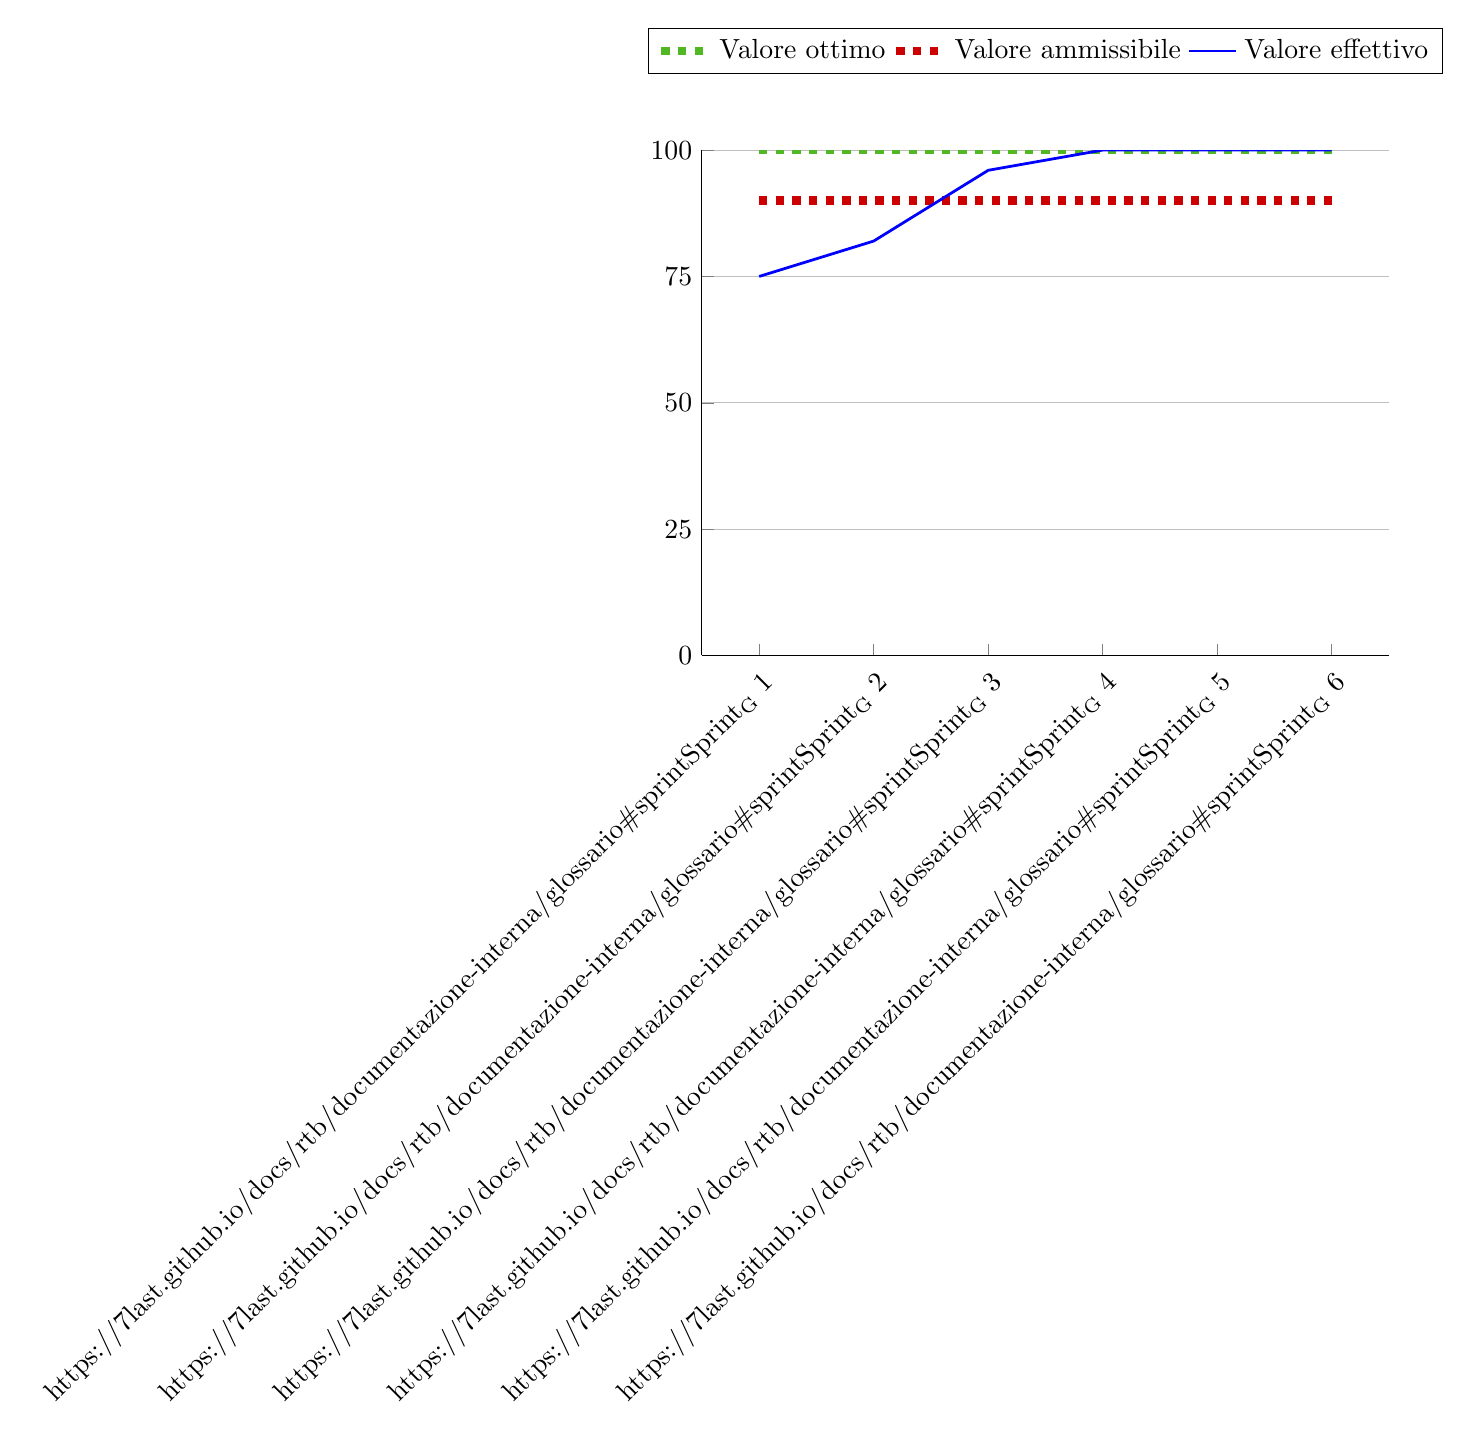
\begin{tikzpicture}
        \begin{axis}[
            width  = 0.85*\textwidth,
            height = 8cm,
            ymajorgrids = true,
            symbolic x coords={\href{https://7last.github.io/docs/rtb/documentazione-interna/glossario\#sprint}{Sprint\textsubscript{G}} 1, \href{https://7last.github.io/docs/rtb/documentazione-interna/glossario\#sprint}{Sprint\textsubscript{G}} 2, \href{https://7last.github.io/docs/rtb/documentazione-interna/glossario\#sprint}{Sprint\textsubscript{G}} 3, \href{https://7last.github.io/docs/rtb/documentazione-interna/glossario\#sprint}{Sprint\textsubscript{G}} 4, \href{https://7last.github.io/docs/rtb/documentazione-interna/glossario\#sprint}{Sprint\textsubscript{G}} 5, \href{https://7last.github.io/docs/rtb/documentazione-interna/glossario\#sprint}{Sprint\textsubscript{G}} 6},
            xtick = data,
            ytick = {0, 25, 50, 75, 100},
            ymin=0, ymax=100,
            axis lines*=left,
            legend cell align=left,
            legend style={
                at={(0.5,1.15)},
                anchor=south,
                column sep=0.1ex,
                legend columns=3
            },
            xticklabel style={rotate=45, anchor=north east, yshift=0ex, xshift=0ex}
        ]
            \addplot[color=opt, style={dashed, line width=3pt}, mark=none] coordinates {(\href{https://7last.github.io/docs/rtb/documentazione-interna/glossario\#sprint}{Sprint\textsubscript{G}} 1, 100) (\href{https://7last.github.io/docs/rtb/documentazione-interna/glossario\#sprint}{Sprint\textsubscript{G}} 2, 100) (\href{https://7last.github.io/docs/rtb/documentazione-interna/glossario\#sprint}{Sprint\textsubscript{G}} 3, 100) (\href{https://7last.github.io/docs/rtb/documentazione-interna/glossario\#sprint}{Sprint\textsubscript{G}} 4, 100) (\href{https://7last.github.io/docs/rtb/documentazione-interna/glossario\#sprint}{Sprint\textsubscript{G}} 5, 100) (\href{https://7last.github.io/docs/rtb/documentazione-interna/glossario\#sprint}{Sprint\textsubscript{G}} 6, 100)}; % ottimo = 100
            \addplot[color=amm, style={dashed, line width=3pt}, mark=none] coordinates {(\href{https://7last.github.io/docs/rtb/documentazione-interna/glossario\#sprint}{Sprint\textsubscript{G}} 1, 90) (\href{https://7last.github.io/docs/rtb/documentazione-interna/glossario\#sprint}{Sprint\textsubscript{G}} 2, 90) (\href{https://7last.github.io/docs/rtb/documentazione-interna/glossario\#sprint}{Sprint\textsubscript{G}} 3, 90) (\href{https://7last.github.io/docs/rtb/documentazione-interna/glossario\#sprint}{Sprint\textsubscript{G}} 4, 90) (\href{https://7last.github.io/docs/rtb/documentazione-interna/glossario\#sprint}{Sprint\textsubscript{G}} 5, 90) (\href{https://7last.github.io/docs/rtb/documentazione-interna/glossario\#sprint}{Sprint\textsubscript{G}} 6, 90)}; % ammissibile = 90
            \addplot[color=blue, style={line width=1pt}, mark=none] coordinates {(\href{https://7last.github.io/docs/rtb/documentazione-interna/glossario\#sprint}{Sprint\textsubscript{G}} 1, 75) (\href{https://7last.github.io/docs/rtb/documentazione-interna/glossario\#sprint}{Sprint\textsubscript{G}} 2, 82) (\href{https://7last.github.io/docs/rtb/documentazione-interna/glossario\#sprint}{Sprint\textsubscript{G}} 3, 96) (\href{https://7last.github.io/docs/rtb/documentazione-interna/glossario\#sprint}{Sprint\textsubscript{G}} 4, 100) (\href{https://7last.github.io/docs/rtb/documentazione-interna/glossario\#sprint}{Sprint\textsubscript{G}} 5, 100) (\href{https://7last.github.io/docs/rtb/documentazione-interna/glossario\#sprint}{Sprint\textsubscript{G}} 6, 100)};
            \legend{Valore ottimo, Valore ammissibile, Valore effettivo}
        \end{axis}
    \end{tikzpicture}
    \caption{Percentuale di metriche di qualità soddisfatte}
\end{figure*}
%--------- FINE GRAFICO -----------%
\subsubsection*{\href{https://7last.github.io/docs/rtb/documentazione-interna/glossario\#requirements-and-technology-baseline}{RTB\textsubscript{G}}}
Osservando il grafico si può notare come inizialmente il valore delle metriche soddisfatte sia inferiore al valore ammissibile, questo è dovuto principalmente all'inesperienza del team. Successivamente l'andamento cresce progressivamente fino ad arrivare al 100\% nell'ultimo \href{https://7last.github.io/docs/rtb/documentazione-interna/glossario\#sprint}{sprint\textsubscript{G}}. Questo indica un miglioramento proressivo del \textit{Way of Working} del gruppo.

%TODO mettere considerazioni finali \href{https://7last.github.io/docs/rtb/documentazione-interna/glossario\#product-baseline}{PB\textsubscript{G}}

% \newpage
% \subsection{Qualità del processo di Verifica}
% \subsubsection{26M-CC - Code coverage}
% %Da qui in poi byteops fanno da "periodo 6"
% %--------- GRAFICO -----------%
% \begin{figure*}[!h]
%     \centering
%     \begin{tikzpicture}
%         \begin{axis}[
%             width  = 0.85*\textwidth,
%             height = 8cm,
%             ymajorgrids = true,
%             symbolic x coords={\href{https://7last.github.io/docs/rtb/documentazione-interna/glossario\#sprint}{Sprint\textsubscript{G}} 1, \href{https://7last.github.io/docs/rtb/documentazione-interna/glossario\#sprint}{Sprint\textsubscript{G}} 2, \href{https://7last.github.io/docs/rtb/documentazione-interna/glossario\#sprint}{Sprint\textsubscript{G}} 3, \href{https://7last.github.io/docs/rtb/documentazione-interna/glossario\#sprint}{Sprint\textsubscript{G}} 4},
%             xtick = data,
%             ytick = {0, 25, 50, 75, 100},
%             ymin=0, ymax=100,
%             axis lines*=left,
%             legend cell align=left,
%             legend style={
%                 at={(0.5,1.15)},
%                 anchor=south,
%                 column sep=0.1ex,
%                 legend columns=-1
%             },
%             xticklabel style={rotate=45, anchor=north east, yshift=0ex, xshift=0ex}
%             ]
%             \addplot[color=opt, style={dashed, line width=3pt}, mark=none] coordinates {(\href{https://7last.github.io/docs/rtb/documentazione-interna/glossario\#sprint}{Sprint\textsubscript{G}} 1, 100) (\href{https://7last.github.io/docs/rtb/documentazione-interna/glossario\#sprint}{Sprint\textsubscript{G}} 2, 100) (\href{https://7last.github.io/docs/rtb/documentazione-interna/glossario\#sprint}{Sprint\textsubscript{G}} 3, 100) (\href{https://7last.github.io/docs/rtb/documentazione-interna/glossario\#sprint}{Sprint\textsubscript{G}} 4, 100)};
%             \addplot[color=amm, style={dashed, line width=3pt}, mark=none] coordinates {(\href{https://7last.github.io/docs/rtb/documentazione-interna/glossario\#sprint}{Sprint\textsubscript{G}} 1, 80) (\href{https://7last.github.io/docs/rtb/documentazione-interna/glossario\#sprint}{Sprint\textsubscript{G}} 2, 80) (\href{https://7last.github.io/docs/rtb/documentazione-interna/glossario\#sprint}{Sprint\textsubscript{G}} 3, 80) (\href{https://7last.github.io/docs/rtb/documentazione-interna/glossario\#sprint}{Sprint\textsubscript{G}} 4, 80)};
%             \addplot[color=blue, style={line width=1pt}, mark=none] coordinates {(\href{https://7last.github.io/docs/rtb/documentazione-interna/glossario\#sprint}{Sprint\textsubscript{G}} 1, 0) (\href{https://7last.github.io/docs/rtb/documentazione-interna/glossario\#sprint}{Sprint\textsubscript{G}} 2, 0) (\href{https://7last.github.io/docs/rtb/documentazione-interna/glossario\#sprint}{Sprint\textsubscript{G}} 3, 0) (\href{https://7last.github.io/docs/rtb/documentazione-interna/glossario\#sprint}{Sprint\textsubscript{G}} 4, 0)};
%             \legend{Valore ottimo, Valore ammissibile, Valore effettivo}
%         \end{axis}
%     \end{tikzpicture}
%     \caption{Percentuale di code coverage dei test implementati}
% \end{figure*}
% %--------- FINE GRAFICO -----------%
% % \subsubsection*{\href{https://7last.github.io/docs/rtb/documentazione-interna/glossario\#requirements-and-technology-baseline}{RTB\textsubscript{G}}}


% %TODO mettere considerazioni finali \href{https://7last.github.io/docs/rtb/documentazione-interna/glossario\#product-baseline}{PB\textsubscript{G}}

% \newpage
% \subsubsection{27M-BC - Branch coverage}
% %--------- GRAFICO -----------%
% \begin{figure*}[!h]
%     \centering
%     \begin{tikzpicture}
%         \begin{axis}[
%             width  = 0.85*\textwidth,
%             height = 8cm,
%             ymajorgrids = true,
%             symbolic x coords={\href{https://7last.github.io/docs/rtb/documentazione-interna/glossario\#sprint}{Sprint\textsubscript{G}} 1, \href{https://7last.github.io/docs/rtb/documentazione-interna/glossario\#sprint}{Sprint\textsubscript{G}} 2, \href{https://7last.github.io/docs/rtb/documentazione-interna/glossario\#sprint}{Sprint\textsubscript{G}} 3, \href{https://7last.github.io/docs/rtb/documentazione-interna/glossario\#sprint}{Sprint\textsubscript{G}} 4},
%             xtick = data,
%             ytick = {0, 25, 50, 75, 100},
%             ymin=0, ymax=100,
%             axis lines*=left,
%             legend cell align=left,
%             legend style={
%                 at={(0.5,1.15)},
%                 anchor=south,
%                 column sep=0.1ex,
%                 legend columns=3
%             },
%             xticklabel style={rotate=45, anchor=north east, yshift=0ex, xshift=0ex}
%             ]
%             \addplot[color=opt, style={dashed, line width=3pt}, mark=none] coordinates {(\href{https://7last.github.io/docs/rtb/documentazione-interna/glossario\#sprint}{Sprint\textsubscript{G}} 1, 100) (\href{https://7last.github.io/docs/rtb/documentazione-interna/glossario\#sprint}{Sprint\textsubscript{G}} 2, 100) (\href{https://7last.github.io/docs/rtb/documentazione-interna/glossario\#sprint}{Sprint\textsubscript{G}} 3, 100) (\href{https://7last.github.io/docs/rtb/documentazione-interna/glossario\#sprint}{Sprint\textsubscript{G}} 4, 100)};
%             \addplot[color=amm, style={dashed, line width=3pt}, mark=none] coordinates {(\href{https://7last.github.io/docs/rtb/documentazione-interna/glossario\#sprint}{Sprint\textsubscript{G}} 1, 80) (\href{https://7last.github.io/docs/rtb/documentazione-interna/glossario\#sprint}{Sprint\textsubscript{G}} 2, 80) (\href{https://7last.github.io/docs/rtb/documentazione-interna/glossario\#sprint}{Sprint\textsubscript{G}} 3, 80) (\href{https://7last.github.io/docs/rtb/documentazione-interna/glossario\#sprint}{Sprint\textsubscript{G}} 4, 80)};
%             \addplot[color=blue, style={line width=1pt}, mark=none] coordinates {(\href{https://7last.github.io/docs/rtb/documentazione-interna/glossario\#sprint}{Sprint\textsubscript{G}} 1, 0) (\href{https://7last.github.io/docs/rtb/documentazione-interna/glossario\#sprint}{Sprint\textsubscript{G}} 2, 0) (\href{https://7last.github.io/docs/rtb/documentazione-interna/glossario\#sprint}{Sprint\textsubscript{G}} 3, 0) (\href{https://7last.github.io/docs/rtb/documentazione-interna/glossario\#sprint}{Sprint\textsubscript{G}} 4, 0)};
%             \legend{Valore ottimo, Valore ammissibile, Valore effettivo}
%         \end{axis}
%     \end{tikzpicture}
%     \caption{Percentuale di branch coverage dei test implementati}
% \end{figure*}
% %--------- FINE GRAFICO -----------%
% % \subsubsection*{\href{https://7last.github.io/docs/rtb/documentazione-interna/glossario\#requirements-and-technology-baseline}{RTB\textsubscript{G}}}

% %TODO mettere considerazioni finali \href{https://7last.github.io/docs/rtb/documentazione-interna/glossario\#product-baseline}{PB\textsubscript{G}}
% \newpage
% \subsubsection{28M-SC - Statement coverage}
% %--------- GRAFICO -----------%
% \begin{figure*}[!h]
%     \centering
%     \begin{tikzpicture}
%         \begin{axis}[
%             width  = 0.85*\textwidth,
%             height = 8cm,
%             ymajorgrids = true,
%             symbolic x coords={\href{https://7last.github.io/docs/rtb/documentazione-interna/glossario\#sprint}{Sprint\textsubscript{G}} 1, \href{https://7last.github.io/docs/rtb/documentazione-interna/glossario\#sprint}{Sprint\textsubscript{G}} 2, \href{https://7last.github.io/docs/rtb/documentazione-interna/glossario\#sprint}{Sprint\textsubscript{G}} 3, \href{https://7last.github.io/docs/rtb/documentazione-interna/glossario\#sprint}{Sprint\textsubscript{G}} 4},
%             xtick = data,
%             ytick = {0, 25, 50, 75, 100},
%             ymin=0, ymax=100,
%             axis lines*=left,
%             legend cell align=left,
%             legend style={
%                 at={(0.5,1.15)},
%                 anchor=south,
%                 column sep=0.1ex,
%                 legend columns=3
%             },
%             xticklabel style={rotate=45, anchor=north east, yshift=0ex, xshift=0ex}
%             ]
%             \addplot[color=opt, style={dashed, line width=3pt}, mark=none] coordinates {(\href{https://7last.github.io/docs/rtb/documentazione-interna/glossario\#sprint}{Sprint\textsubscript{G}} 1, 100) (\href{https://7last.github.io/docs/rtb/documentazione-interna/glossario\#sprint}{Sprint\textsubscript{G}} 2, 100) (\href{https://7last.github.io/docs/rtb/documentazione-interna/glossario\#sprint}{Sprint\textsubscript{G}} 3, 100) (\href{https://7last.github.io/docs/rtb/documentazione-interna/glossario\#sprint}{Sprint\textsubscript{G}} 4, 100)};
%             \addplot[color=amm, style={dashed, line width=3pt}, mark=none] coordinates {(\href{https://7last.github.io/docs/rtb/documentazione-interna/glossario\#sprint}{Sprint\textsubscript{G}} 1, 80) (\href{https://7last.github.io/docs/rtb/documentazione-interna/glossario\#sprint}{Sprint\textsubscript{G}} 2, 80) (\href{https://7last.github.io/docs/rtb/documentazione-interna/glossario\#sprint}{Sprint\textsubscript{G}} 3, 80) (\href{https://7last.github.io/docs/rtb/documentazione-interna/glossario\#sprint}{Sprint\textsubscript{G}} 4, 80)};
%             \addplot[color=blue, style={line width=1pt}, mark=none] coordinates {(\href{https://7last.github.io/docs/rtb/documentazione-interna/glossario\#sprint}{Sprint\textsubscript{G}} 1, 0) (\href{https://7last.github.io/docs/rtb/documentazione-interna/glossario\#sprint}{Sprint\textsubscript{G}} 2, 0) (\href{https://7last.github.io/docs/rtb/documentazione-interna/glossario\#sprint}{Sprint\textsubscript{G}} 3, 0)  (\href{https://7last.github.io/docs/rtb/documentazione-interna/glossario\#sprint}{Sprint\textsubscript{G}} 4, 0)};
%             \legend{Valore ottimo, Valore ammissibile, Valore effettivo}
%         \end{axis}
%     \end{tikzpicture}
%     \caption{Percentuale di statement coverage dei test implementati}
% \end{figure*}
% %--------- FINE GRAFICO -----------%
% % \subsubsection*{\href{https://7last.github.io/docs/rtb/documentazione-interna/glossario\#requirements-and-technology-baseline}{RTB\textsubscript{G}}}

% %TODO mettere considerazioni finali \href{https://7last.github.io/docs/rtb/documentazione-interna/glossario\#product-baseline}{PB\textsubscript{G}}
% \newpage
% \subsubsection{29M-FD - Failure density}
% %--------- GRAFICO -----------%
% \begin{figure*}[!h]
%     \centering
%     \begin{tikzpicture}
%         \begin{axis}[
%             width  = 0.85*\textwidth,
%             height = 8cm,
%             ymajorgrids = true,
%             symbolic x coords={\href{https://7last.github.io/docs/rtb/documentazione-interna/glossario\#sprint}{Sprint\textsubscript{G}} 1, \href{https://7last.github.io/docs/rtb/documentazione-interna/glossario\#sprint}{Sprint\textsubscript{G}} 2, \href{https://7last.github.io/docs/rtb/documentazione-interna/glossario\#sprint}{Sprint\textsubscript{G}} 3, \href{https://7last.github.io/docs/rtb/documentazione-interna/glossario\#sprint}{Sprint\textsubscript{G}} 4},
%             xtick = data,
%             ytick = {0, 25, 50, 75, 100},
%             ymin=0, ymax=100,
%             axis lines*=left,
%             legend cell align=left,
%             legend style={
%                 at={(0.5,1.15)},
%                 anchor=south,
%                 column sep=0.1ex,
%                 legend columns=3
%             },
%             xticklabel style={rotate=45, anchor=north east, yshift=0ex, xshift=0ex}
%             ]
%             \addplot[color=opt, style={dashed, line width=3pt}, mark=none] coordinates {(\href{https://7last.github.io/docs/rtb/documentazione-interna/glossario\#sprint}{Sprint\textsubscript{G}} 1, 0) (\href{https://7last.github.io/docs/rtb/documentazione-interna/glossario\#sprint}{Sprint\textsubscript{G}} 2, 0) (\href{https://7last.github.io/docs/rtb/documentazione-interna/glossario\#sprint}{Sprint\textsubscript{G}} 3, 0) (\href{https://7last.github.io/docs/rtb/documentazione-interna/glossario\#sprint}{Sprint\textsubscript{G}} 4, 0)};
%             \addplot[color=amm, style={dashed, line width=3pt}, mark=none] coordinates {(\href{https://7last.github.io/docs/rtb/documentazione-interna/glossario\#sprint}{Sprint\textsubscript{G}} 1, 15) (\href{https://7last.github.io/docs/rtb/documentazione-interna/glossario\#sprint}{Sprint\textsubscript{G}} 2, 15) (\href{https://7last.github.io/docs/rtb/documentazione-interna/glossario\#sprint}{Sprint\textsubscript{G}} 3, 15) (\href{https://7last.github.io/docs/rtb/documentazione-interna/glossario\#sprint}{Sprint\textsubscript{G}} 4, 15)};
%             \addplot[color=blue, style={line width=1pt}, mark=none] coordinates {(\href{https://7last.github.io/docs/rtb/documentazione-interna/glossario\#sprint}{Sprint\textsubscript{G}} 1, 0) (\href{https://7last.github.io/docs/rtb/documentazione-interna/glossario\#sprint}{Sprint\textsubscript{G}} 2, 0) (\href{https://7last.github.io/docs/rtb/documentazione-interna/glossario\#sprint}{Sprint\textsubscript{G}} 3, 0) (\href{https://7last.github.io/docs/rtb/documentazione-interna/glossario\#sprint}{Sprint\textsubscript{G}} 4, 0)};
%             \legend{Valore ottimo, Valore ammissibile, Valore effettivo}
%         \end{axis}
%     \end{tikzpicture}
%     \caption{Percentuale di failure density}
% \end{figure*}
% %--------- FINE GRAFICO -----------%
% % \subsubsection*{\href{https://7last.github.io/docs/rtb/documentazione-interna/glossario\#requirements-and-technology-baseline}{RTB\textsubscript{G}}}

% %TODO mettere considerazioni finali \href{https://7last.github.io/docs/rtb/documentazione-interna/glossario\#product-baseline}{PB\textsubscript{G}}

% \newpage
% \subsubsection{30M-PTCP - Passed Test Case Percentage}
% %--------- GRAFICO -----------%
% \begin{figure*}[!h]
%     \centering
%     \begin{tikzpicture}
%         \begin{axis}[
%             width  = 0.85*\textwidth,
%             height = 8cm,
%             ymajorgrids = true,
%             symbolic x coords={\href{https://7last.github.io/docs/rtb/documentazione-interna/glossario\#sprint}{Sprint\textsubscript{G}} 1, \href{https://7last.github.io/docs/rtb/documentazione-interna/glossario\#sprint}{Sprint\textsubscript{G}} 2, \href{https://7last.github.io/docs/rtb/documentazione-interna/glossario\#sprint}{Sprint\textsubscript{G}} 3, \href{https://7last.github.io/docs/rtb/documentazione-interna/glossario\#sprint}{Sprint\textsubscript{G}} 4},
%             xtick = data,
%             ytick = {0, 25, 50, 75, 100},
%             ymin=0, ymax=100,
%             axis lines*=left,
%             legend cell align=left,
%             legend style={
%                 at={(0.5,1.15)},
%                 anchor=south,
%                 column sep=0.1ex,
%                 legend columns=3
%             },
%             xticklabel style={rotate=45, anchor=north east, yshift=0ex, xshift=0ex}
%             ]
%             \addplot[color=opt, style={dashed, line width=3pt}, mark=none] coordinates {(\href{https://7last.github.io/docs/rtb/documentazione-interna/glossario\#sprint}{Sprint\textsubscript{G}} 1, 100) (\href{https://7last.github.io/docs/rtb/documentazione-interna/glossario\#sprint}{Sprint\textsubscript{G}} 2, 100) (\href{https://7last.github.io/docs/rtb/documentazione-interna/glossario\#sprint}{Sprint\textsubscript{G}} 3, 100) (\href{https://7last.github.io/docs/rtb/documentazione-interna/glossario\#sprint}{Sprint\textsubscript{G}} 4, 100)};
%             \addplot[color=amm, style={dashed, line width=3pt}, mark=none] coordinates {(\href{https://7last.github.io/docs/rtb/documentazione-interna/glossario\#sprint}{Sprint\textsubscript{G}} 1, 90) (\href{https://7last.github.io/docs/rtb/documentazione-interna/glossario\#sprint}{Sprint\textsubscript{G}} 2, 90) (\href{https://7last.github.io/docs/rtb/documentazione-interna/glossario\#sprint}{Sprint\textsubscript{G}} 3, 90) (\href{https://7last.github.io/docs/rtb/documentazione-interna/glossario\#sprint}{Sprint\textsubscript{G}} 4, 90)};
%             \addplot[color=blue, style={line width=1pt}, mark=none] coordinates {(\href{https://7last.github.io/docs/rtb/documentazione-interna/glossario\#sprint}{Sprint\textsubscript{G}} 1, 0) (\href{https://7last.github.io/docs/rtb/documentazione-interna/glossario\#sprint}{Sprint\textsubscript{G}} 2, 0) (\href{https://7last.github.io/docs/rtb/documentazione-interna/glossario\#sprint}{Sprint\textsubscript{G}} 3, 0) (\href{https://7last.github.io/docs/rtb/documentazione-interna/glossario\#sprint}{Sprint\textsubscript{G}} 4, 0)};
%             \legend{Valore ottimo, Valore ammissibile, Valore effettivo}
%         \end{axis}
%     \end{tikzpicture}
%     \caption{Percentuale di casi di test superati}
% \end{figure*}
% %--------- FINE GRAFICO -----------%
% \subsubsection*{\href{https://7last.github.io/docs/rtb/documentazione-interna/glossario\#requirements-and-technology-baseline}{RTB\textsubscript{G}}}

% %TODO mettere considerazioni finali \href{https://7last.github.io/docs/rtb/documentazione-interna/glossario\#product-baseline}{PB\textsubscript{G}}
\newpage
\subsection{Qualità del processo di Gestione dei rischi}
\subsubsection{32M-NCR - Rischi Non Calcolati}
%--------- GRAFICO -----------%
\begin{figure*}[!h]
    \centering
    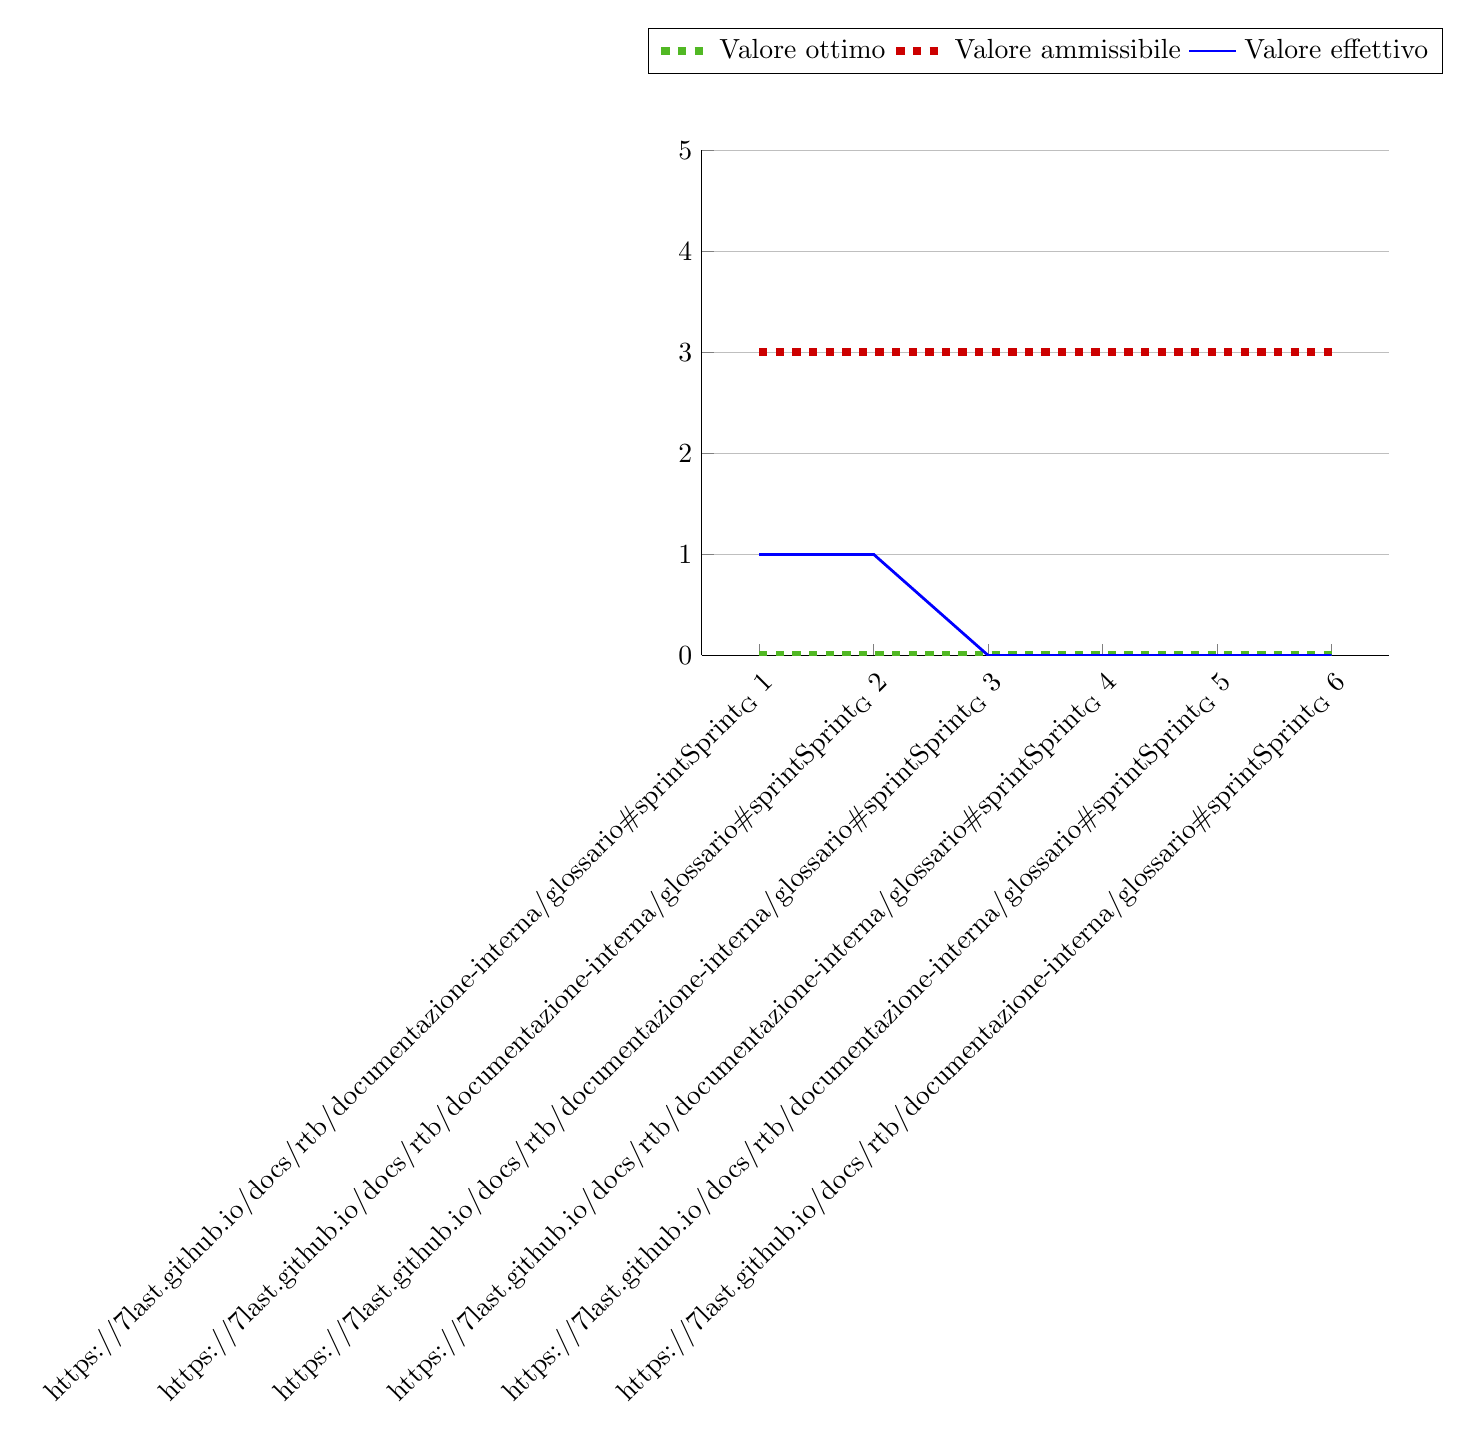
\begin{tikzpicture}
        \begin{axis}[
            width  = 0.85*\textwidth,
            height = 8cm,
            ymajorgrids = true,
            symbolic x coords={\href{https://7last.github.io/docs/rtb/documentazione-interna/glossario\#sprint}{Sprint\textsubscript{G}} 1, \href{https://7last.github.io/docs/rtb/documentazione-interna/glossario\#sprint}{Sprint\textsubscript{G}} 2, \href{https://7last.github.io/docs/rtb/documentazione-interna/glossario\#sprint}{Sprint\textsubscript{G}} 3, \href{https://7last.github.io/docs/rtb/documentazione-interna/glossario\#sprint}{Sprint\textsubscript{G}} 4, \href{https://7last.github.io/docs/rtb/documentazione-interna/glossario\#sprint}{Sprint\textsubscript{G}} 5, \href{https://7last.github.io/docs/rtb/documentazione-interna/glossario\#sprint}{Sprint\textsubscript{G}} 6},
            xtick = data,
            ymin=0, ymax=5,
            axis lines*=left,
            legend cell align=left,
            legend style={
                at={(0.5,1.15)},
                anchor=south,
                column sep=0.1ex,
                legend columns=3
            },
            xticklabel style={rotate=45, anchor=north east, yshift=0ex, xshift=0ex}
        ]
            \addplot[color=opt, style={dashed, line width=3pt}, mark=none] coordinates {(\href{https://7last.github.io/docs/rtb/documentazione-interna/glossario\#sprint}{Sprint\textsubscript{G}} 1, 0) (\href{https://7last.github.io/docs/rtb/documentazione-interna/glossario\#sprint}{Sprint\textsubscript{G}} 2, 0) (\href{https://7last.github.io/docs/rtb/documentazione-interna/glossario\#sprint}{Sprint\textsubscript{G}} 3, 0) (\href{https://7last.github.io/docs/rtb/documentazione-interna/glossario\#sprint}{Sprint\textsubscript{G}} 4, 0) (\href{https://7last.github.io/docs/rtb/documentazione-interna/glossario\#sprint}{Sprint\textsubscript{G}} 5, 0) (\href{https://7last.github.io/docs/rtb/documentazione-interna/glossario\#sprint}{Sprint\textsubscript{G}} 6, 0)}; % ottimo = 0
            \addplot[color=amm, style={dashed, line width=3pt}, mark=none] coordinates {(\href{https://7last.github.io/docs/rtb/documentazione-interna/glossario\#sprint}{Sprint\textsubscript{G}} 1, 3) (\href{https://7last.github.io/docs/rtb/documentazione-interna/glossario\#sprint}{Sprint\textsubscript{G}} 2, 3) (\href{https://7last.github.io/docs/rtb/documentazione-interna/glossario\#sprint}{Sprint\textsubscript{G}} 3, 3) (\href{https://7last.github.io/docs/rtb/documentazione-interna/glossario\#sprint}{Sprint\textsubscript{G}} 4, 3) (\href{https://7last.github.io/docs/rtb/documentazione-interna/glossario\#sprint}{Sprint\textsubscript{G}} 5, 3) (\href{https://7last.github.io/docs/rtb/documentazione-interna/glossario\#sprint}{Sprint\textsubscript{G}} 6, 3)}; % ammissibile = 3
            \addplot[color=blue, style={line width=1pt}, mark=none] coordinates {(\href{https://7last.github.io/docs/rtb/documentazione-interna/glossario\#sprint}{Sprint\textsubscript{G}} 1, 1) (\href{https://7last.github.io/docs/rtb/documentazione-interna/glossario\#sprint}{Sprint\textsubscript{G}} 2, 1) (\href{https://7last.github.io/docs/rtb/documentazione-interna/glossario\#sprint}{Sprint\textsubscript{G}} 3, 0) (\href{https://7last.github.io/docs/rtb/documentazione-interna/glossario\#sprint}{Sprint\textsubscript{G}} 4, 0) (\href{https://7last.github.io/docs/rtb/documentazione-interna/glossario\#sprint}{Sprint\textsubscript{G}} 5, 0) (\href{https://7last.github.io/docs/rtb/documentazione-interna/glossario\#sprint}{Sprint\textsubscript{G}} 6, 0)}; % rischi non calcolati
            \legend{Valore ottimo, Valore ammissibile, Valore effettivo}
        \end{axis}
    \end{tikzpicture}
    \caption{Rischi non calcolati occorsi durante il progetto}
\end{figure*}
%--------- FINE GRAFICO -----------%
\subsubsection*{\href{https://7last.github.io/docs/rtb/documentazione-interna/glossario\#requirements-and-technology-baseline}{RTB\textsubscript{G}}}
Dal grafico si evince che durante i primi \href{https://7last.github.io/docs/rtb/documentazione-interna/glossario\#sprint}{sprint\textsubscript{G}} sono emersi rischi non calcolati, sintomo di una pianificazione non ottimale dovuta all'inesperienza. Successivamente il team ha accumulato esperienza, mediante automiglioramento, imparando a gestire e prevenire i rischi in modo migliore.
%TODO mettere considerazioni finali \href{https://7last.github.io/docs/rtb/documentazione-interna/glossario\#product-baseline}{PB\textsubscript{G}}

\newpage
\subsection{Qualità del processo di Pianificazione}
\subsubsection{33M-RSI - Requirements Stability Index}
%--------- GRAFICO -----------%
\begin{figure*}[!h]
    \centering
    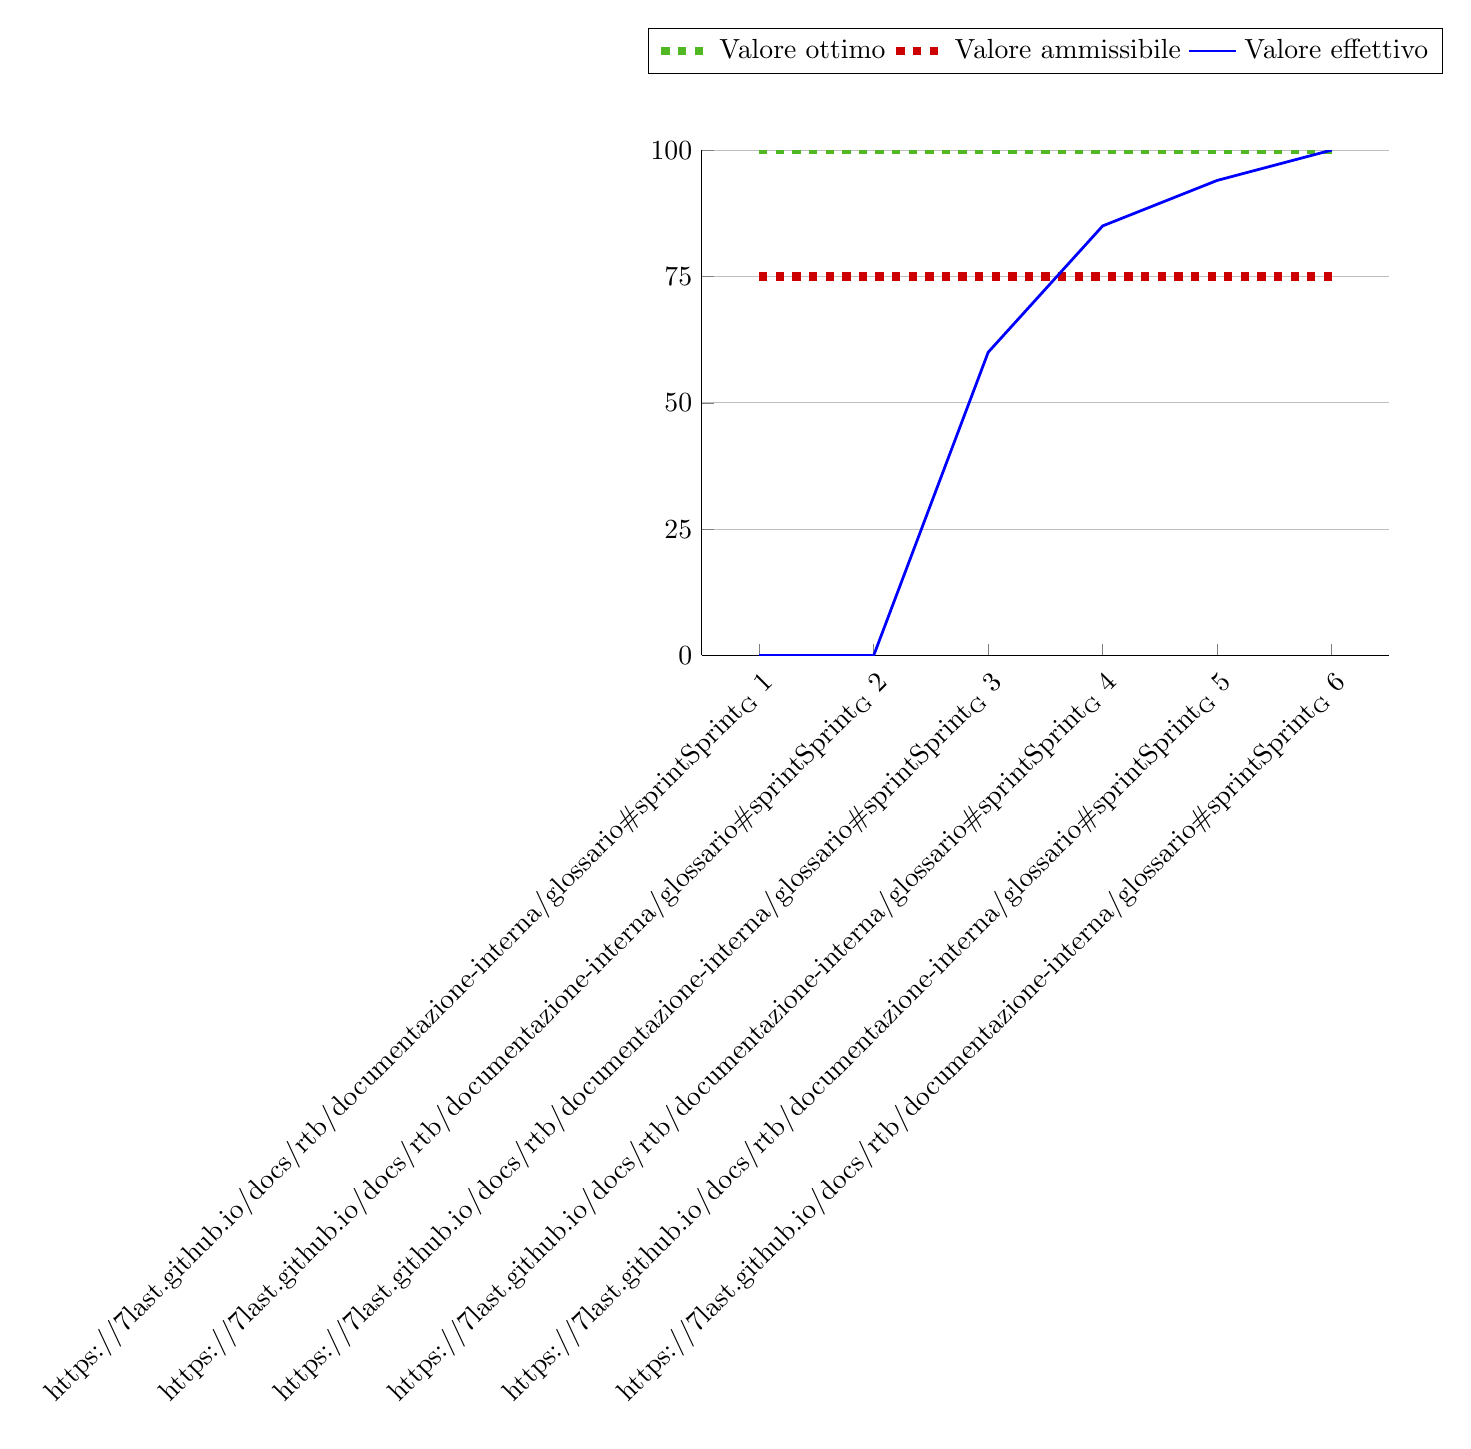
\begin{tikzpicture}
        \begin{axis}[
            width  = 0.85*\textwidth,
            height = 8cm,
            ymajorgrids = true,
            symbolic x coords={\href{https://7last.github.io/docs/rtb/documentazione-interna/glossario\#sprint}{Sprint\textsubscript{G}} 1, \href{https://7last.github.io/docs/rtb/documentazione-interna/glossario\#sprint}{Sprint\textsubscript{G}} 2, \href{https://7last.github.io/docs/rtb/documentazione-interna/glossario\#sprint}{Sprint\textsubscript{G}} 3, \href{https://7last.github.io/docs/rtb/documentazione-interna/glossario\#sprint}{Sprint\textsubscript{G}} 4, \href{https://7last.github.io/docs/rtb/documentazione-interna/glossario\#sprint}{Sprint\textsubscript{G}} 5, \href{https://7last.github.io/docs/rtb/documentazione-interna/glossario\#sprint}{Sprint\textsubscript{G}} 6},
            xtick = data,
            ytick = {0, 25, 50, 75, 100},
            ymin=0, ymax=100,
            axis lines*=left,
            legend cell align=left,
            legend style={
                at={(0.5,1.15)},
                anchor=south,
                column sep=0.1ex,
                legend columns=3
            },
            xticklabel style={rotate=45, anchor=north east, yshift=0ex, xshift=0ex}
        ]
            \addplot[color=opt, style={dashed, line width=3pt}, mark=none] coordinates {(\href{https://7last.github.io/docs/rtb/documentazione-interna/glossario\#sprint}{Sprint\textsubscript{G}} 1, 100) (\href{https://7last.github.io/docs/rtb/documentazione-interna/glossario\#sprint}{Sprint\textsubscript{G}} 2, 100) (\href{https://7last.github.io/docs/rtb/documentazione-interna/glossario\#sprint}{Sprint\textsubscript{G}} 3, 100) (\href{https://7last.github.io/docs/rtb/documentazione-interna/glossario\#sprint}{Sprint\textsubscript{G}} 4, 100) (\href{https://7last.github.io/docs/rtb/documentazione-interna/glossario\#sprint}{Sprint\textsubscript{G}} 5, 100) (\href{https://7last.github.io/docs/rtb/documentazione-interna/glossario\#sprint}{Sprint\textsubscript{G}} 6, 100)}; % ottimo = 100
            \addplot[color=amm, style={dashed, line width=3pt}, mark=none] coordinates {(\href{https://7last.github.io/docs/rtb/documentazione-interna/glossario\#sprint}{Sprint\textsubscript{G}} 1, 75) (\href{https://7last.github.io/docs/rtb/documentazione-interna/glossario\#sprint}{Sprint\textsubscript{G}} 2, 75) (\href{https://7last.github.io/docs/rtb/documentazione-interna/glossario\#sprint}{Sprint\textsubscript{G}} 3, 75) (\href{https://7last.github.io/docs/rtb/documentazione-interna/glossario\#sprint}{Sprint\textsubscript{G}} 4, 75) (\href{https://7last.github.io/docs/rtb/documentazione-interna/glossario\#sprint}{Sprint\textsubscript{G}} 5, 75) (\href{https://7last.github.io/docs/rtb/documentazione-interna/glossario\#sprint}{Sprint\textsubscript{G}} 6, 75)}; % ammissibile = 75
            \addplot[color=blue, style={line width=1pt}, mark=none] coordinates {(\href{https://7last.github.io/docs/rtb/documentazione-interna/glossario\#sprint}{Sprint\textsubscript{G}} 1, 0) (\href{https://7last.github.io/docs/rtb/documentazione-interna/glossario\#sprint}{Sprint\textsubscript{G}} 2, 0) (\href{https://7last.github.io/docs/rtb/documentazione-interna/glossario\#sprint}{Sprint\textsubscript{G}} 3, 60) (\href{https://7last.github.io/docs/rtb/documentazione-interna/glossario\#sprint}{Sprint\textsubscript{G}} 4, 85) (\href{https://7last.github.io/docs/rtb/documentazione-interna/glossario\#sprint}{Sprint\textsubscript{G}} 5, 94) (\href{https://7last.github.io/docs/rtb/documentazione-interna/glossario\#sprint}{Sprint\textsubscript{G}} 6, 100)}; % RSI
            \legend{Valore ottimo, Valore ammissibile, Valore effettivo}
        \end{axis}
    \end{tikzpicture}
    \caption{Percentuale di stabilità dei requisiti}
\end{figure*}
%--------- FINE GRAFICO -----------%
\subsubsection*{\href{https://7last.github.io/docs/rtb/documentazione-interna/glossario\#requirements-and-technology-baseline}{RTB\textsubscript{G}}}
L'analisi del RSI mostra un forte incremento tra il secondo e il terzo \href{https://7last.github.io/docs/rtb/documentazione-interna/glossario\#sprint}{sprint\textsubscript{G}}, segnalando un'intensa attività di revisione e aggiustamento dei requisiti. Nei due \href{https://7last.github.io/docs/rtb/documentazione-interna/glossario\#sprint}{sprint\textsubscript{G}} successivi, il RSI si stabilizza, indicando una riduzione delle modifiche e una maggiore stabilità dei requisiti. Questo andamento riflette un'efficace fase iniziale di consolidamento dei requisiti seguita da una stabilizzazione che facilita l'implementazione del progetto.
%TODO mettere considerazioni finali \href{https://7last.github.io/docs/rtb/documentazione-interna/glossario\#product-baseline}{PB\textsubscript{G}}
